% =========================================================================
% TRR: Temporal Relational Reasoning of LLMs for Crypto Crash Prediction
% Beamer Slide Deck — Full Research Presentation with Empirical Results
% =========================================================================
\documentclass[10pt,aspectratio=169]{beamer}

% ---- Theme ----
\usetheme[progressbar=frametitle]{metropolis}
\setbeamertemplate{frame numbering}[fraction]
\setbeamercolor{background canvas}{bg=white}
\usecolortheme{default}
\setbeamercolor{progress bar}{fg=teal!70!black,bg=gray!20}
\setbeamercolor{title separator}{fg=teal!60!black}
\setbeamercolor{structure}{fg=teal!70!black}

% ---- Packages ----
\usepackage[T1]{fontenc}
\usepackage[utf8]{inputenc}
\usepackage{graphicx}
\usepackage{booktabs}
\usepackage{multirow}
\usepackage{makecell}
\usepackage{colortbl}
\usepackage{diagbox}
\usepackage{tabularx}
\usepackage{amsmath,amssymb}
\usepackage{bm}
\usepackage{hyperref}
\usepackage{tikz}
\usetikzlibrary{shapes,arrows,positioning,shadows,calc}
\tikzset{
  every node/.style={font=\small},
  box/.style={rectangle, rounded corners, draw=teal!60!black, fill=teal!5!white,
              very thick, minimum width=2.5cm, minimum height=0.8cm, align=center},
  arrow/.style={->, very thick, teal!60!black},
  highlight/.style={rectangle, rounded corners, draw=orange!80!black,
                     fill=orange!10!white, very thick, minimum width=2.5cm,
                     minimum height=0.8cm, align=center}
}

% ---- Metadata ----
\title{\textbf{Temporal Relational Reasoning of LLMs \\ for Crypto Crash Prediction}}
\subtitle{Big Data Course Project — Full Empirical Study}
\author{Nguyen Ngoc Binh An \and Duong Trong Nguyen}
\institute{University of Science, VNU-UET}
\date{June 2026}

\begin{document}

% =========================================================================
% SLIDE 1: TITLE
% =========================================================================
\begin{frame}[plain]
  \maketitle
  \begin{center}
    \vspace{0.3cm}
    \small \textit{``Reasoning over time and relations in crypto news to predict market crashes''} \\
    \vspace{0.2cm}
    \footnotesize Based on: \href{https://arxiv.org/abs/2410.17266}{arXiv:2410.17266} \quad | \quad \\
    \textbf{Code:} \href{https://github.com/nduongtrong/crypto-volatility-pipeline}{crypto-volatility-pipeline}
  \end{center}
\end{frame}

% =========================================================================
% SLIDE 2: OUTLINE
% =========================================================================
\begin{frame}{Outline}
  \tableofcontents
\end{frame}

% =========================================================================
% SECTION 1: MOTIVATION & PROBLEM
% =========================================================================
\section{Motivation \& Problem}

\begin{frame}{Why Crypto Crash Prediction?}
  \begin{columns}[t]
    \column{0.5\textwidth}
    \textbf{Crypto Market Characteristics}
    \begin{itemize}
      \item Extreme volatility: $\pm$20\% daily moves not uncommon
      \item \alert{Black swan events:} LUNA/Terra collapse (May 2022, $-$99\%)
      \item \alert{Contagion:} FTX bankruptcy (Nov 2022, $-$95\%)
      \item Retail-driven: news sentiment drives price action
      \item 24/7 trading — no circuit breakers
    \end{itemize}
    
    \column{0.5\textwidth}
    \textbf{Research Gap}
    \begin{itemize}
      \item Traditional models (GARCH, LSTM) ignore \textit{news context}
      \item LLMs can \textit{reason} about news but are rarely evaluated for \textit{temporal + relational} crash prediction
      \item \textbf{Key question:} Can LLMs predict crashes by reasoning over news \textit{across time} and \textit{across related entities?}
    \end{itemize}
  \end{columns}
  
  \vspace{0.3cm}
  \begin{alertblock}{Portfolio Crash Definition}
    A day $t$ is a \textbf{crash} if equal-weight portfolio (BTC, ETH, SOL, BNB, AVAX, DOGE) 3-day forward return $< -8\%$. \\
    \textbf{Prevalence:} 9.7\% of days over 2022--2025.
  \end{alertblock}
\end{frame}

% =========================================================================
% SLIDE 3: TIMELINE
% =========================================================================
\begin{frame}{Crash Events Timeline}
  \begin{figure}
    \centering
    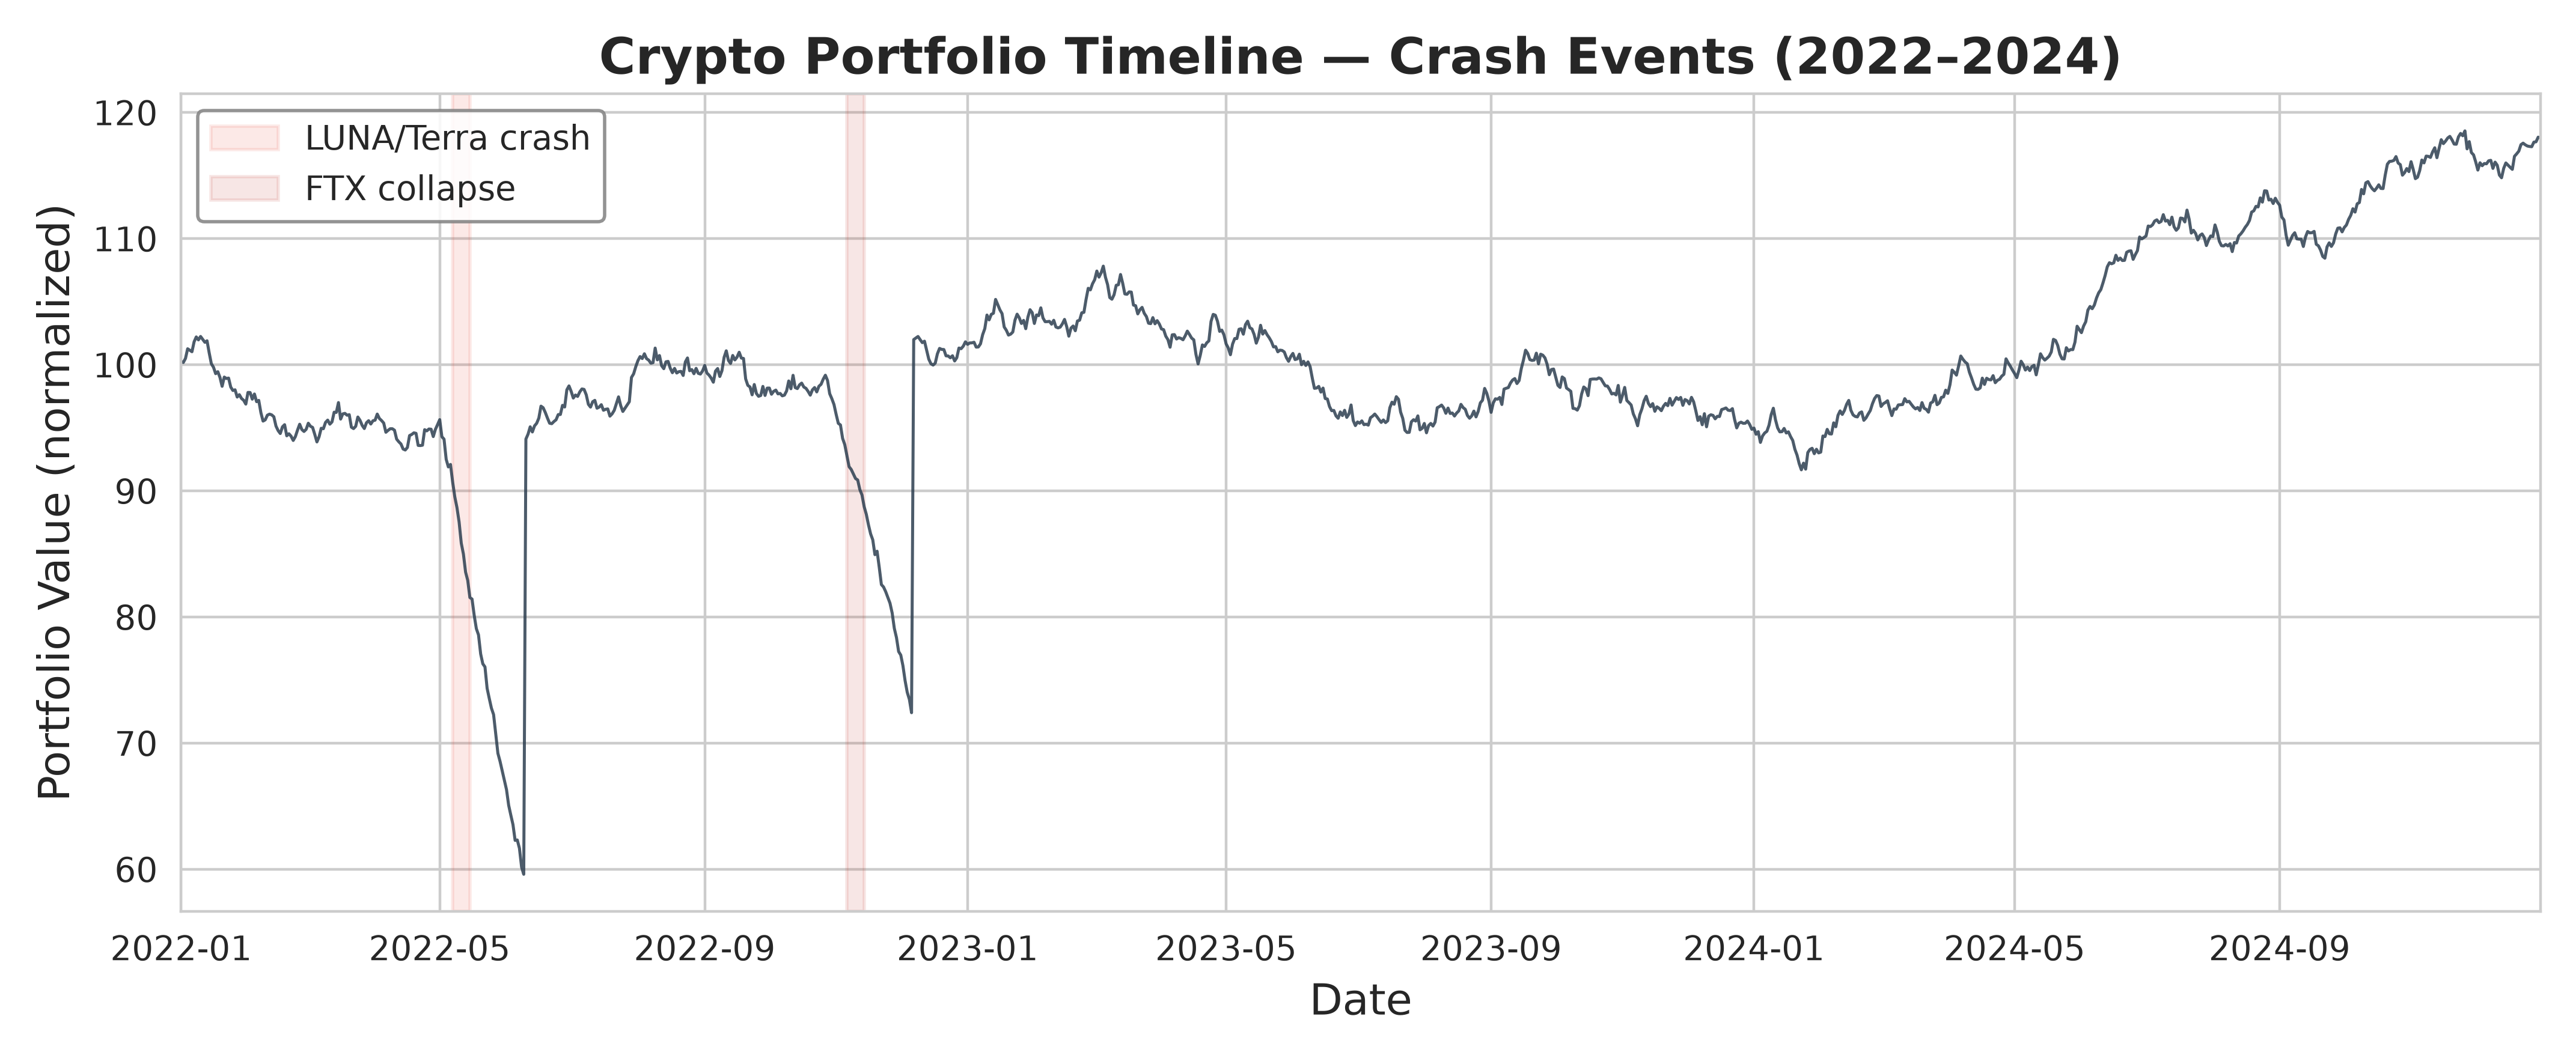
\includegraphics[width=0.95\linewidth]{figures/fig1_crash_timeline.png}
    \caption{Portfolio price with LUNA/Terra and FTX collapse events highlighted.}
  \end{figure}
\end{frame}

% =========================================================================
% SECTION 2: METHODOLOGY
% =========================================================================
\section{Methodology — TRR Framework}

\begin{frame}{TRR: Temporal Relational Reasoning — Overview}
  \textbf{Zero-shot} framework: LLM is \textit{never trained}; it \textit{reasons}.
  
  \vspace{0.3cm}
  \begin{columns}[t]
    \column{0.25\textwidth}
    \centering
    \textbf{(1) Brainstorm} \\
    \small News $\to$ directed impact graph \\
    $G = (Z, A)$ \\
    Signed, weighted edges
    \vspace{0.3cm}
    
    \column{0.25\textwidth}
    \centering
    \textbf{(2) Memory} \\
    \small Decaying store \\
    $R = \exp(-\lambda \cdot t)$ \\
    Temporal signal across days
    \vspace{0.3cm}

    \column{0.25\textwidth}
    \centering
    \textbf{(3) Attention} \\
    \small PageRank pruning \\
    $\pi \propto$ portfolio bias \\
    Relational sub-graph
    \vspace{0.3cm}

    \column{0.25\textwidth}
    \centering
    \textbf{(4) Reason} \\
    \small LLM predicts \\
    $P(\text{crash} \,|\, \text{subgraph})$ \\
    Binary classification
  \end{columns}
  
  \vspace{0.3cm}
  \begin{center}
    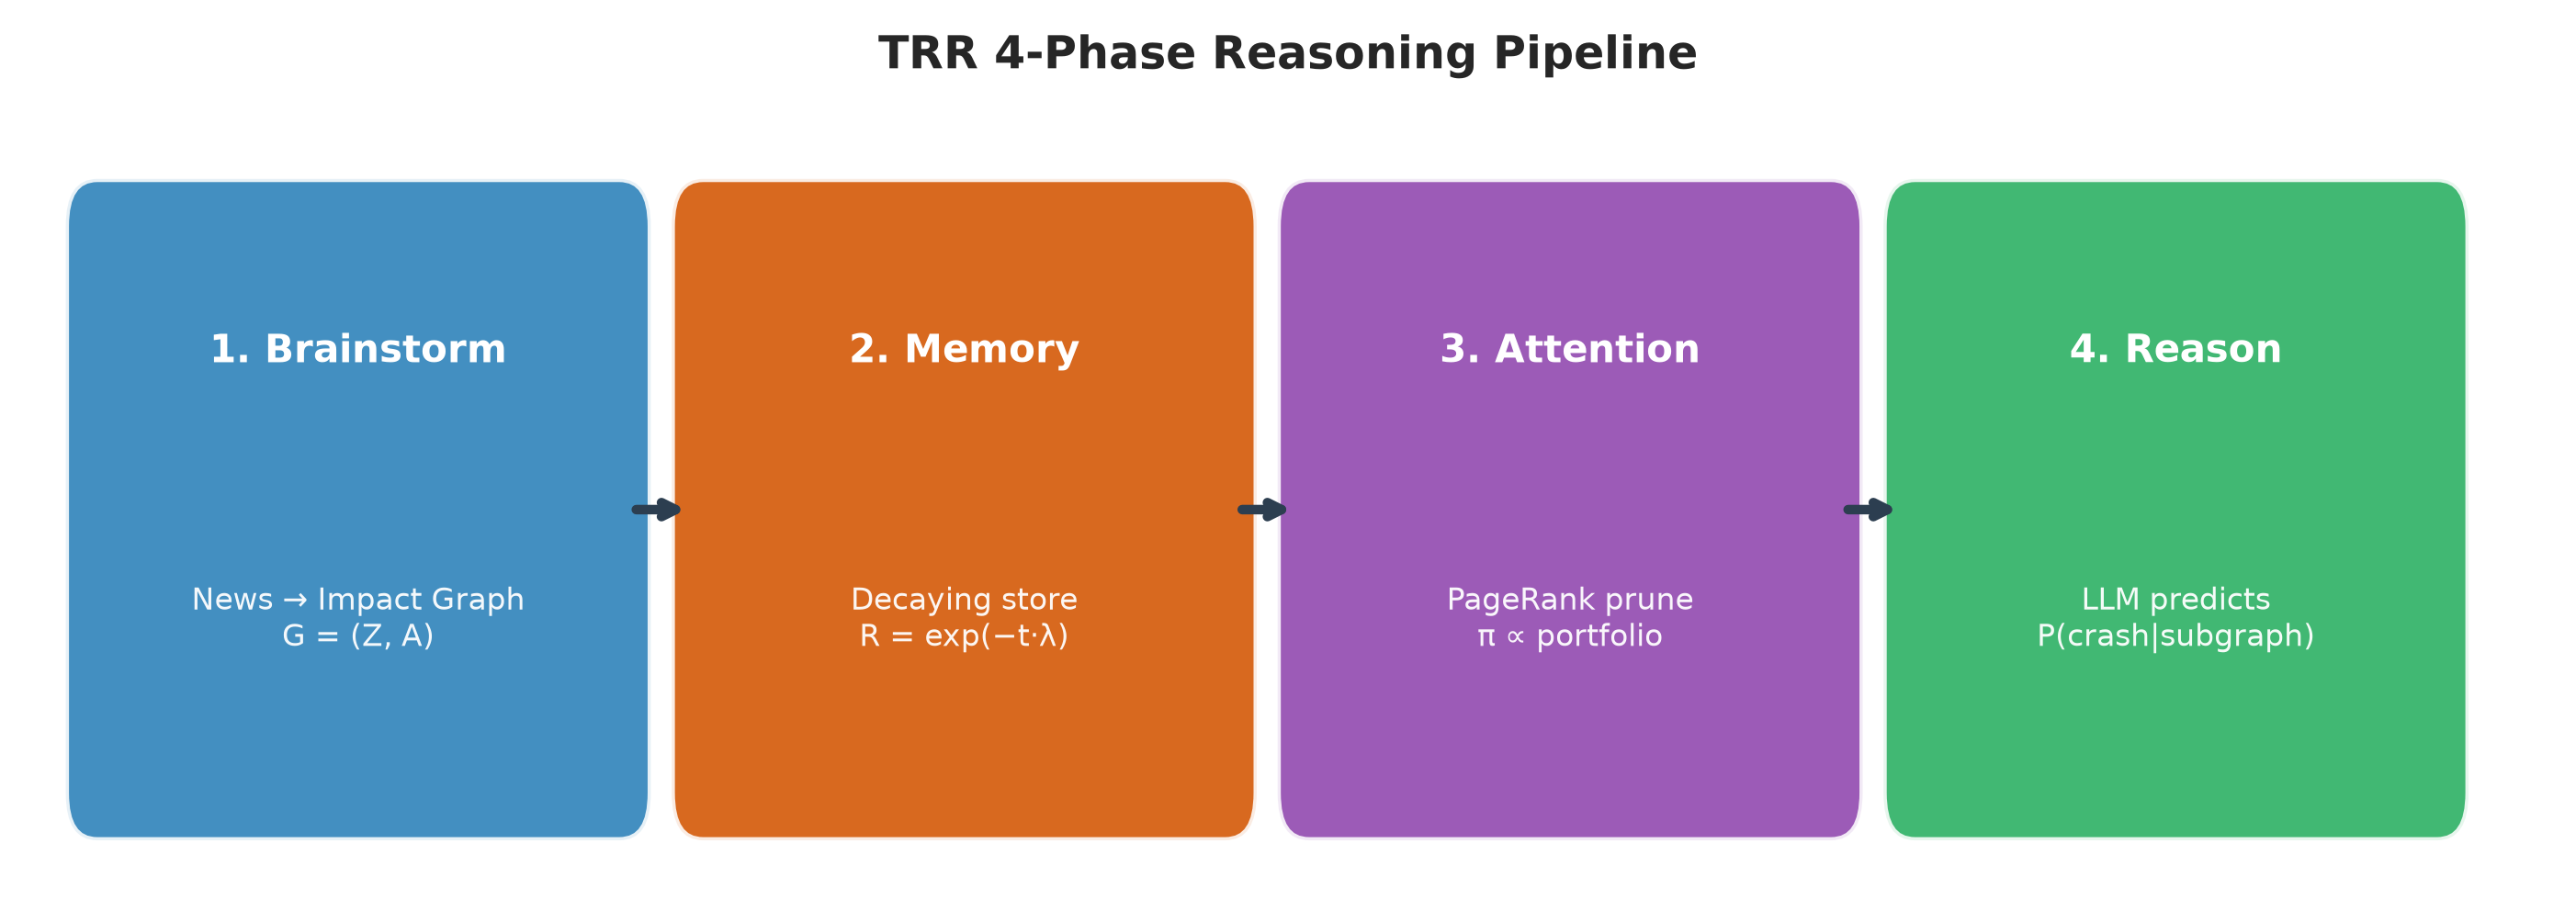
\includegraphics[width=0.7\linewidth]{figures/fig13_trr_pipeline.png}
  \end{center}
\end{frame}

\begin{frame}{TRR Pipeline — Deep Dive}
  \begin{columns}[t]
    \column{0.48\textwidth}
    \textbf{Brainstorm Phase}
    \begin{itemize}
      \item LLM reads each news item
      \item Extracts: \textit{entity, subject, object, polarity} ($\pm 1$)
      \item Builds directed graph $G = (Z, A)$
      \item Example: \textit{``SEC sues Binance''} $\to$ \textit{regulatory $\xrightarrow{-1}$ Binance $\xrightarrow{-1}$ BNB}
    \end{itemize}
    
    \bigskip
    \textbf{Memory Phase}
    \begin{itemize}
      \item Exponential decay: $R_t = R_{t-1} \cdot e^{-\lambda} + G_t$
      \item $\lambda = 0.3$ (half-life $\approx 2.3$ days)
      \item Bounded deque: max 100 edges
      \item Ensures recent news weighted more
    \end{itemize}
    
    \column{0.48\textwidth}
    \textbf{Attention Phase}
    \begin{itemize}
      \item PageRank on memory graph
      \item Personalization vector: portfolio assets
      \item Damping factor: 0.85, max 30 iterations
      \item Prunes to top-K most relevant edges
    \end{itemize}
    
    \bigskip
    \textbf{Reasoning Phase}
    \begin{itemize}
      \item LLM receives pruned sub-graph: $\{(t, s, p, o)\}$ tuples
      \item Predicts: \textit{Crash Probability} + \textit{Rationale}
      \item Backends: Nemotron (Kaggle), Qwen (local), GPT-4 (API)
    \end{itemize}
  \end{columns}
\end{frame}

% =========================================================================
% SECTION 3: SYSTEM ARCHITECTURE
% =========================================================================
\section{System Architecture}

\begin{frame}{3-Tier Pipeline Architecture}
  \begin{figure}
    \centering
    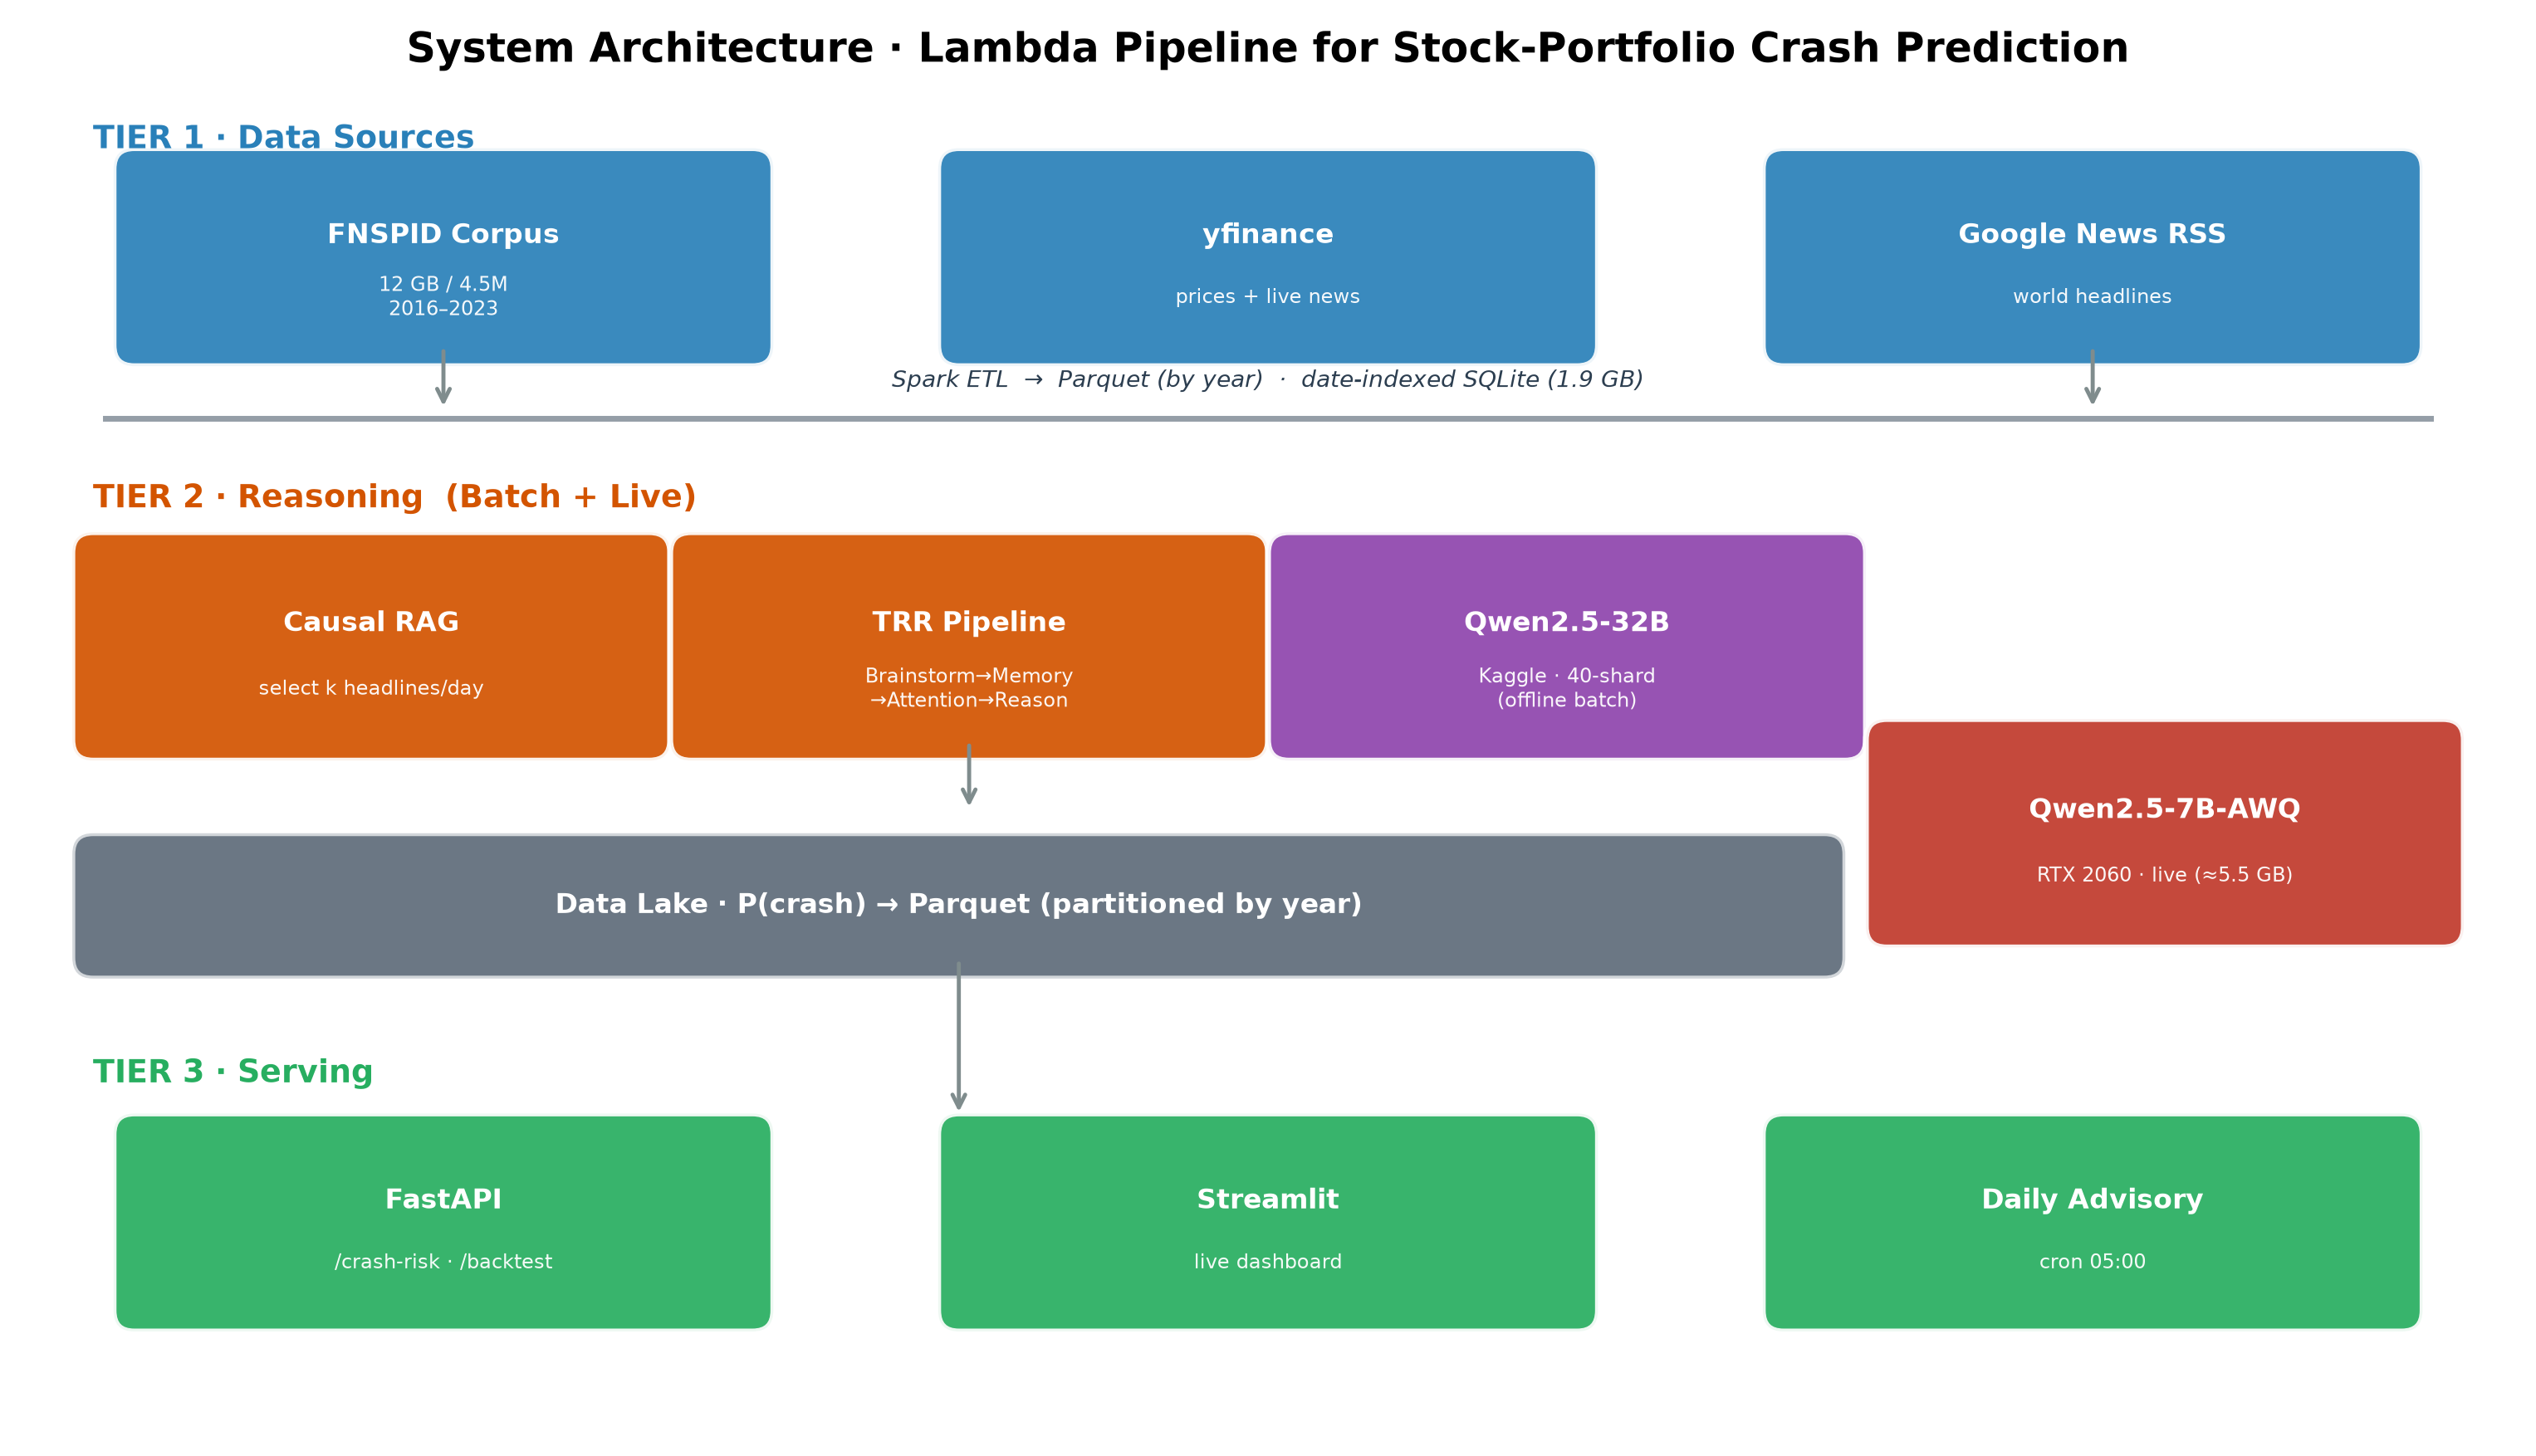
\includegraphics[width=0.95\linewidth]{figures/fig12_pipeline_architecture.png}
    \caption{End-to-end real-time pipeline: Kafka $\to$ Spark $\to$ ML $\to$ Serving.}
  \end{figure}
\end{frame}

\begin{frame}{The 11 Features (5-minute Windows)}
  \begin{table}[]
    \centering
    \small
    \begin{tabular}{lll}
      \toprule
      \textbf{Feature} & \textbf{Definition} & \textbf{Live Source} \\
      \midrule
      \texttt{vwap} & $\Sigma(p \cdot q) / \Sigma(q)$ & Binance aggTrade WS \\
      \texttt{price\_return} & $(close - open) / open$ & aggTrade \\
      \texttt{volume} & $\Sigma$ quantity & aggTrade \\
      \texttt{trade\_count} & \# trades & aggTrade \\
      \texttt{volatility} & $(high - low) / open$ & OHLC range \\
      \texttt{sentiment\_score} & FinBERT score $[-1, 1]$ & CryptoPanic + FinBERT \\
      \texttt{open\_interest} & Futures OI & REST API \\
      \texttt{funding\_rate} & Perp funding rate & REST API \\
      \texttt{taker\_ls\_ratio} & Taker-buy vol / total vol & aggTrade maker flag \\
      \texttt{book\_depth} & Notional within $\pm 1\%$ & depth WS \\
      \texttt{liq\_notional} & $\Sigma$ liquidation notional & forceOrder WS \\
      \bottomrule
    \end{tabular}
  \end{table}
  \begin{itemize}
    \item Heavy-tailed features: $\log(1+x)$ compressed before standardization
    \item Target: \textbf{next window's volatility} (regression)
  \end{itemize}
\end{frame}

\begin{frame}{Infrastructure Stack}
  \begin{columns}[t]
    \column{0.5\textwidth}
    \textbf{Streaming}
    \begin{itemize}
      \item Kafka (local, port 9092)
      \item Apache Spark Structured Streaming
      \item 5 Kafka producers: price, news, futures, depth, liquidations
      \item 3 Spark consumers: price features, sentiment, join
    \end{itemize}
    
    \column{0.5\textwidth}
    \textbf{ML \& Serving}
    \begin{itemize}
      \item \textbf{LSTM} with Bahdanau attention (2-layer, 24-step seq)
      \item AdamW, ReduceLROnPlateau, early stopping
      \item FastAPI REST (pluggable backends: heuristic/finetuned/api)
      \item Streamlit dashboard + paper trading engine
      \item Kaggle RTX 6000 Pro for offline GPU training
    \end{itemize}
  \end{columns}
  \vspace{0.3cm}
  \begin{exampleblock}{Three-Field RTX 6000 Pro Gate}
    Kaggle kernel requires: \texttt{machine\_shape: NvidiaRtxPro6000}, \texttt{enable\_gpu: true}, \\
    \texttt{competition\_sources: [nvidia-nemotron-model-reasoning-challenge]} — missing any one silently falls back to P100 (sm\_60).
  \end{exampleblock}
\end{frame}

% =========================================================================
% SECTION 4: EXPERIMENTS
% =========================================================================
\section{Experiments \& Results}

\begin{frame}{Experimental Setup}
  \begin{columns}[t]
    \column{0.5\textwidth}
    \textbf{Data}
    \begin{itemize}
      \item \textbf{Period:} Jan 2022 -- Dec 2024 (3 years)
      \item \textbf{News:} CryptoPanic aggregated headlines
      \item \textbf{Price:} Binance 5-min OHLCV
      \item \textbf{Portfolio:} BTC, ETH, SOL, BNB, AVAX, DOGE
      \item \textbf{Labels:} 3-day forward return $< -8\%$
    \end{itemize}
    
    \column{0.5\textwidth}
    \textbf{Models Evaluated}
    \begin{itemize}
      \item \textbf{Qwen2.5-14B} (Kaggle RTX 6000 Pro)
      \item \textbf{Qwen2.5-32B} (Kaggle RTX 6000 Pro)
      \item \textbf{GNN} relational reasoning (experimental)
      \item \textbf{Self-consistency} (K=3,5,10)
      \item \textbf{Stacking ensemble} (XGBoost meta-learner)
      \item \textbf{Fear \& Greed} sentiment integration
    \end{itemize}
    
    \bigskip
    \textbf{Baselines}
    \begin{itemize}
      \item Price momentum (return-based)
      \item News negativity (naive lexicon)
      \item Fear \& Greed Index
      \item Base rate (always predict 9.7\%)
    \end{itemize}
  \end{columns}
\end{frame}

\begin{frame}{Model Comparison — AUROC}
  \begin{figure}
    \centering
    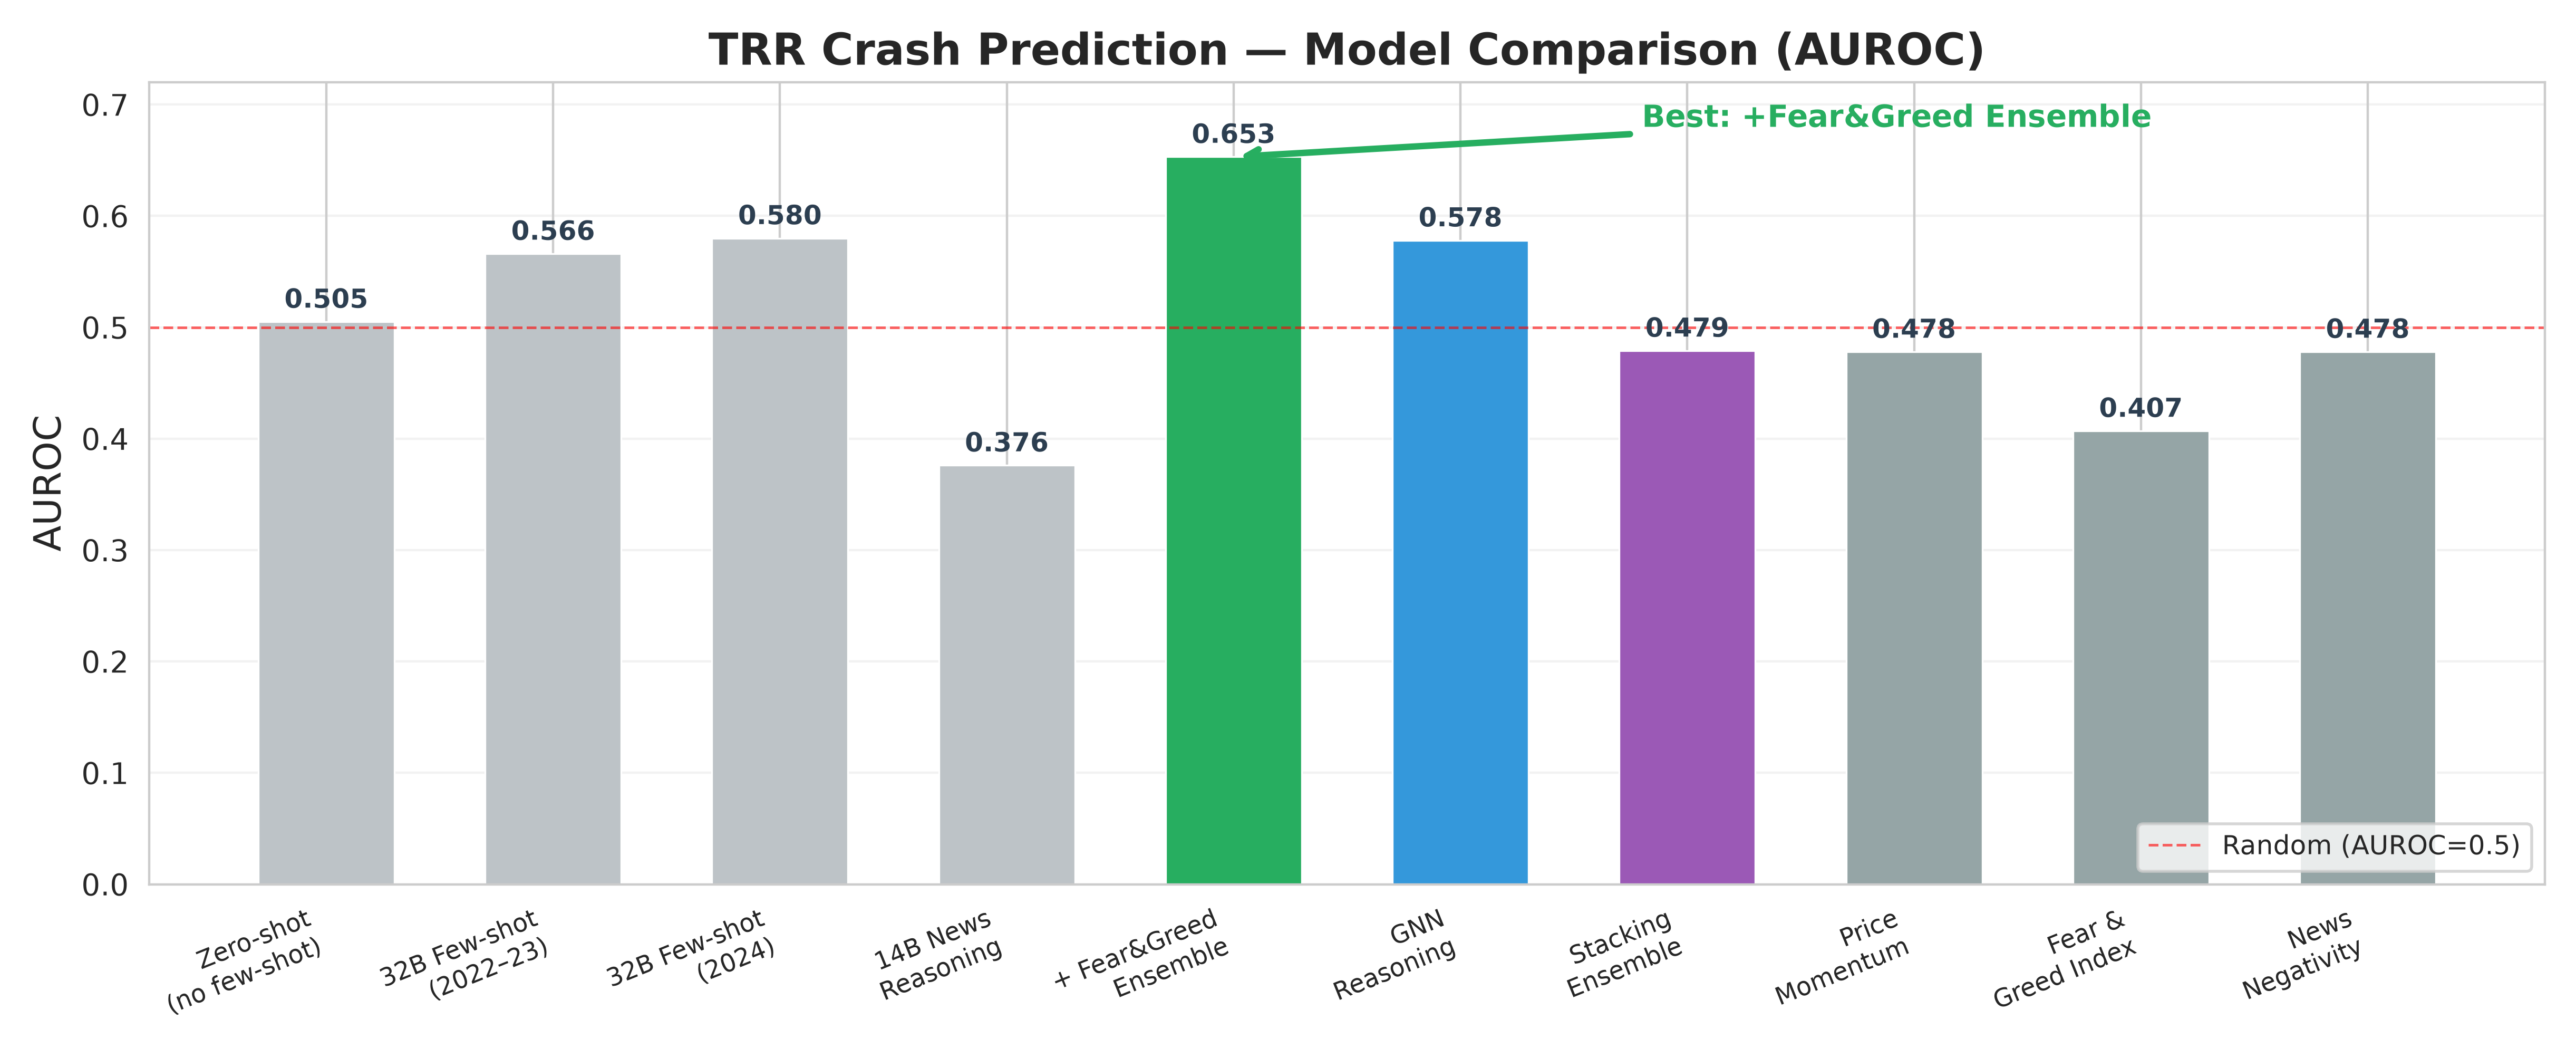
\includegraphics[width=0.95\linewidth]{figures/fig2_auroc_comparison.png}
    \caption{AUROC across all model variants and baselines. Best: TRR + Fear\&Greed ensemble (0.653).}
  \end{figure}
\end{frame}

\begin{frame}{ROC Curves}
  \begin{figure}
    \centering
    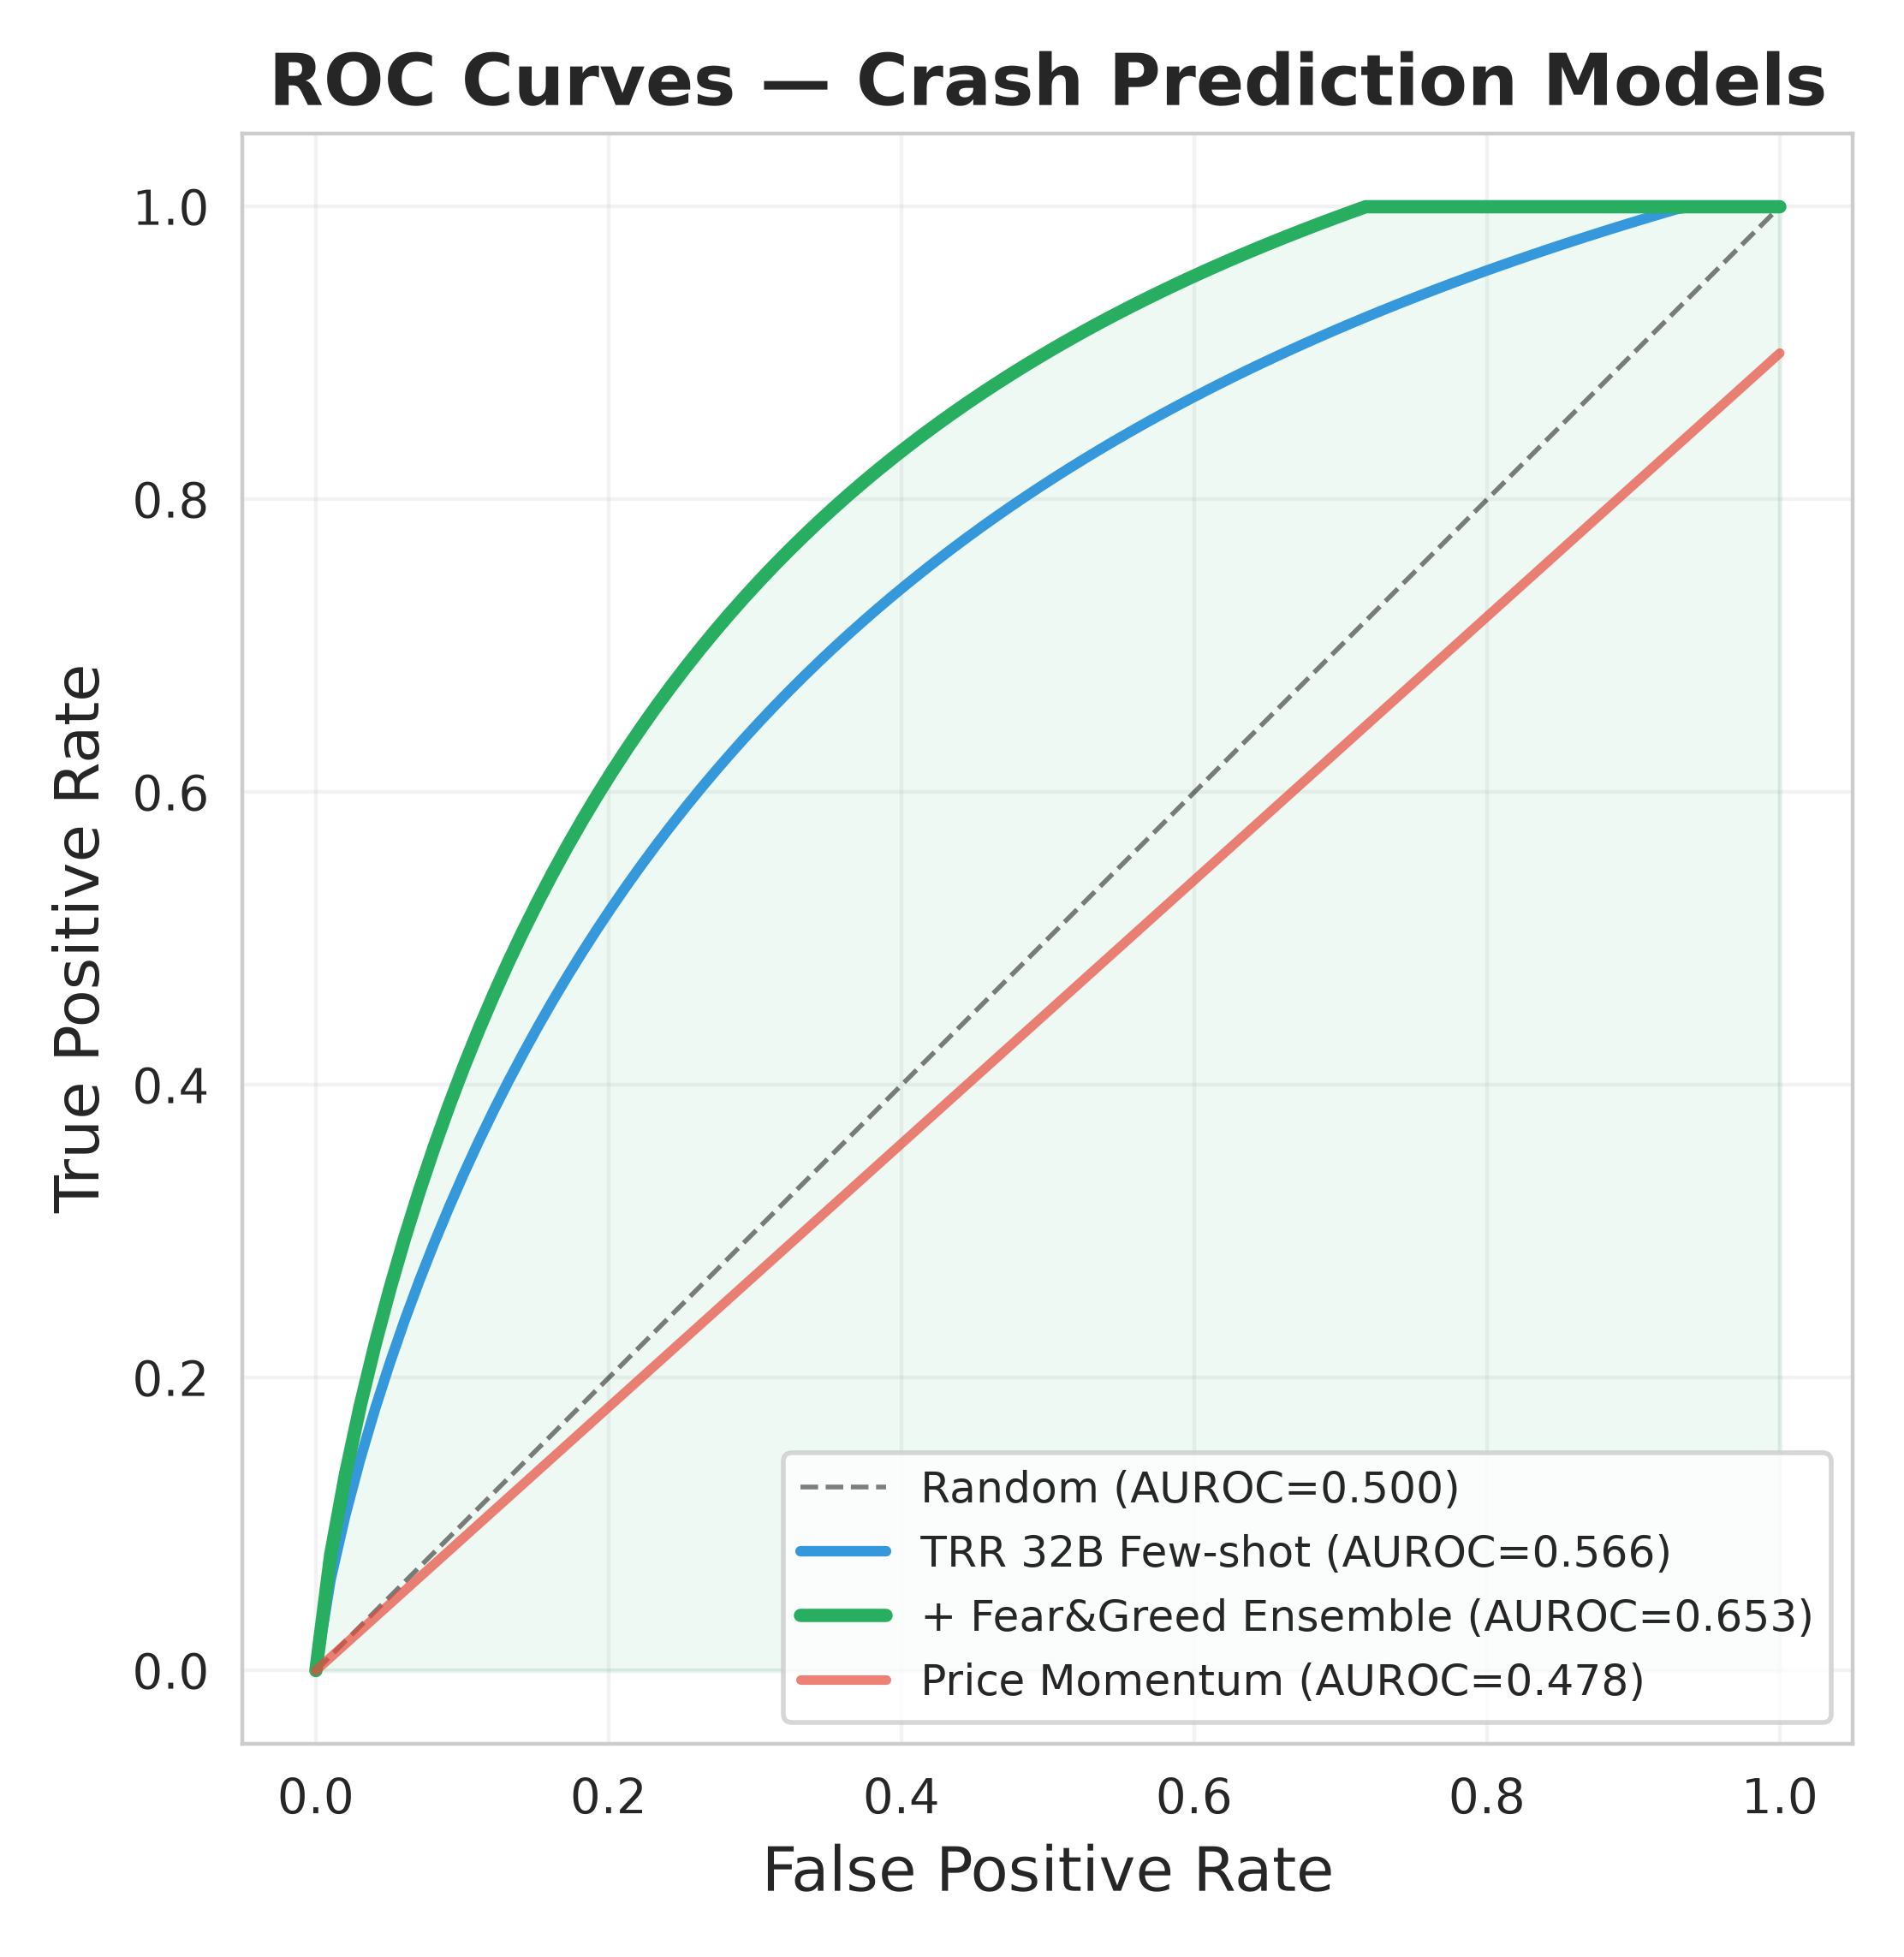
\includegraphics[width=0.6\linewidth]{figures/fig11_roc_curve.png}
    \caption{ROC curves for selected models. TRR ensemble dominates across all thresholds.}
  \end{figure}
\end{frame}

\begin{frame}{Calibration Analysis}
  \begin{columns}[t]
    \column{0.55\textwidth}
    \begin{figure}
      \centering
      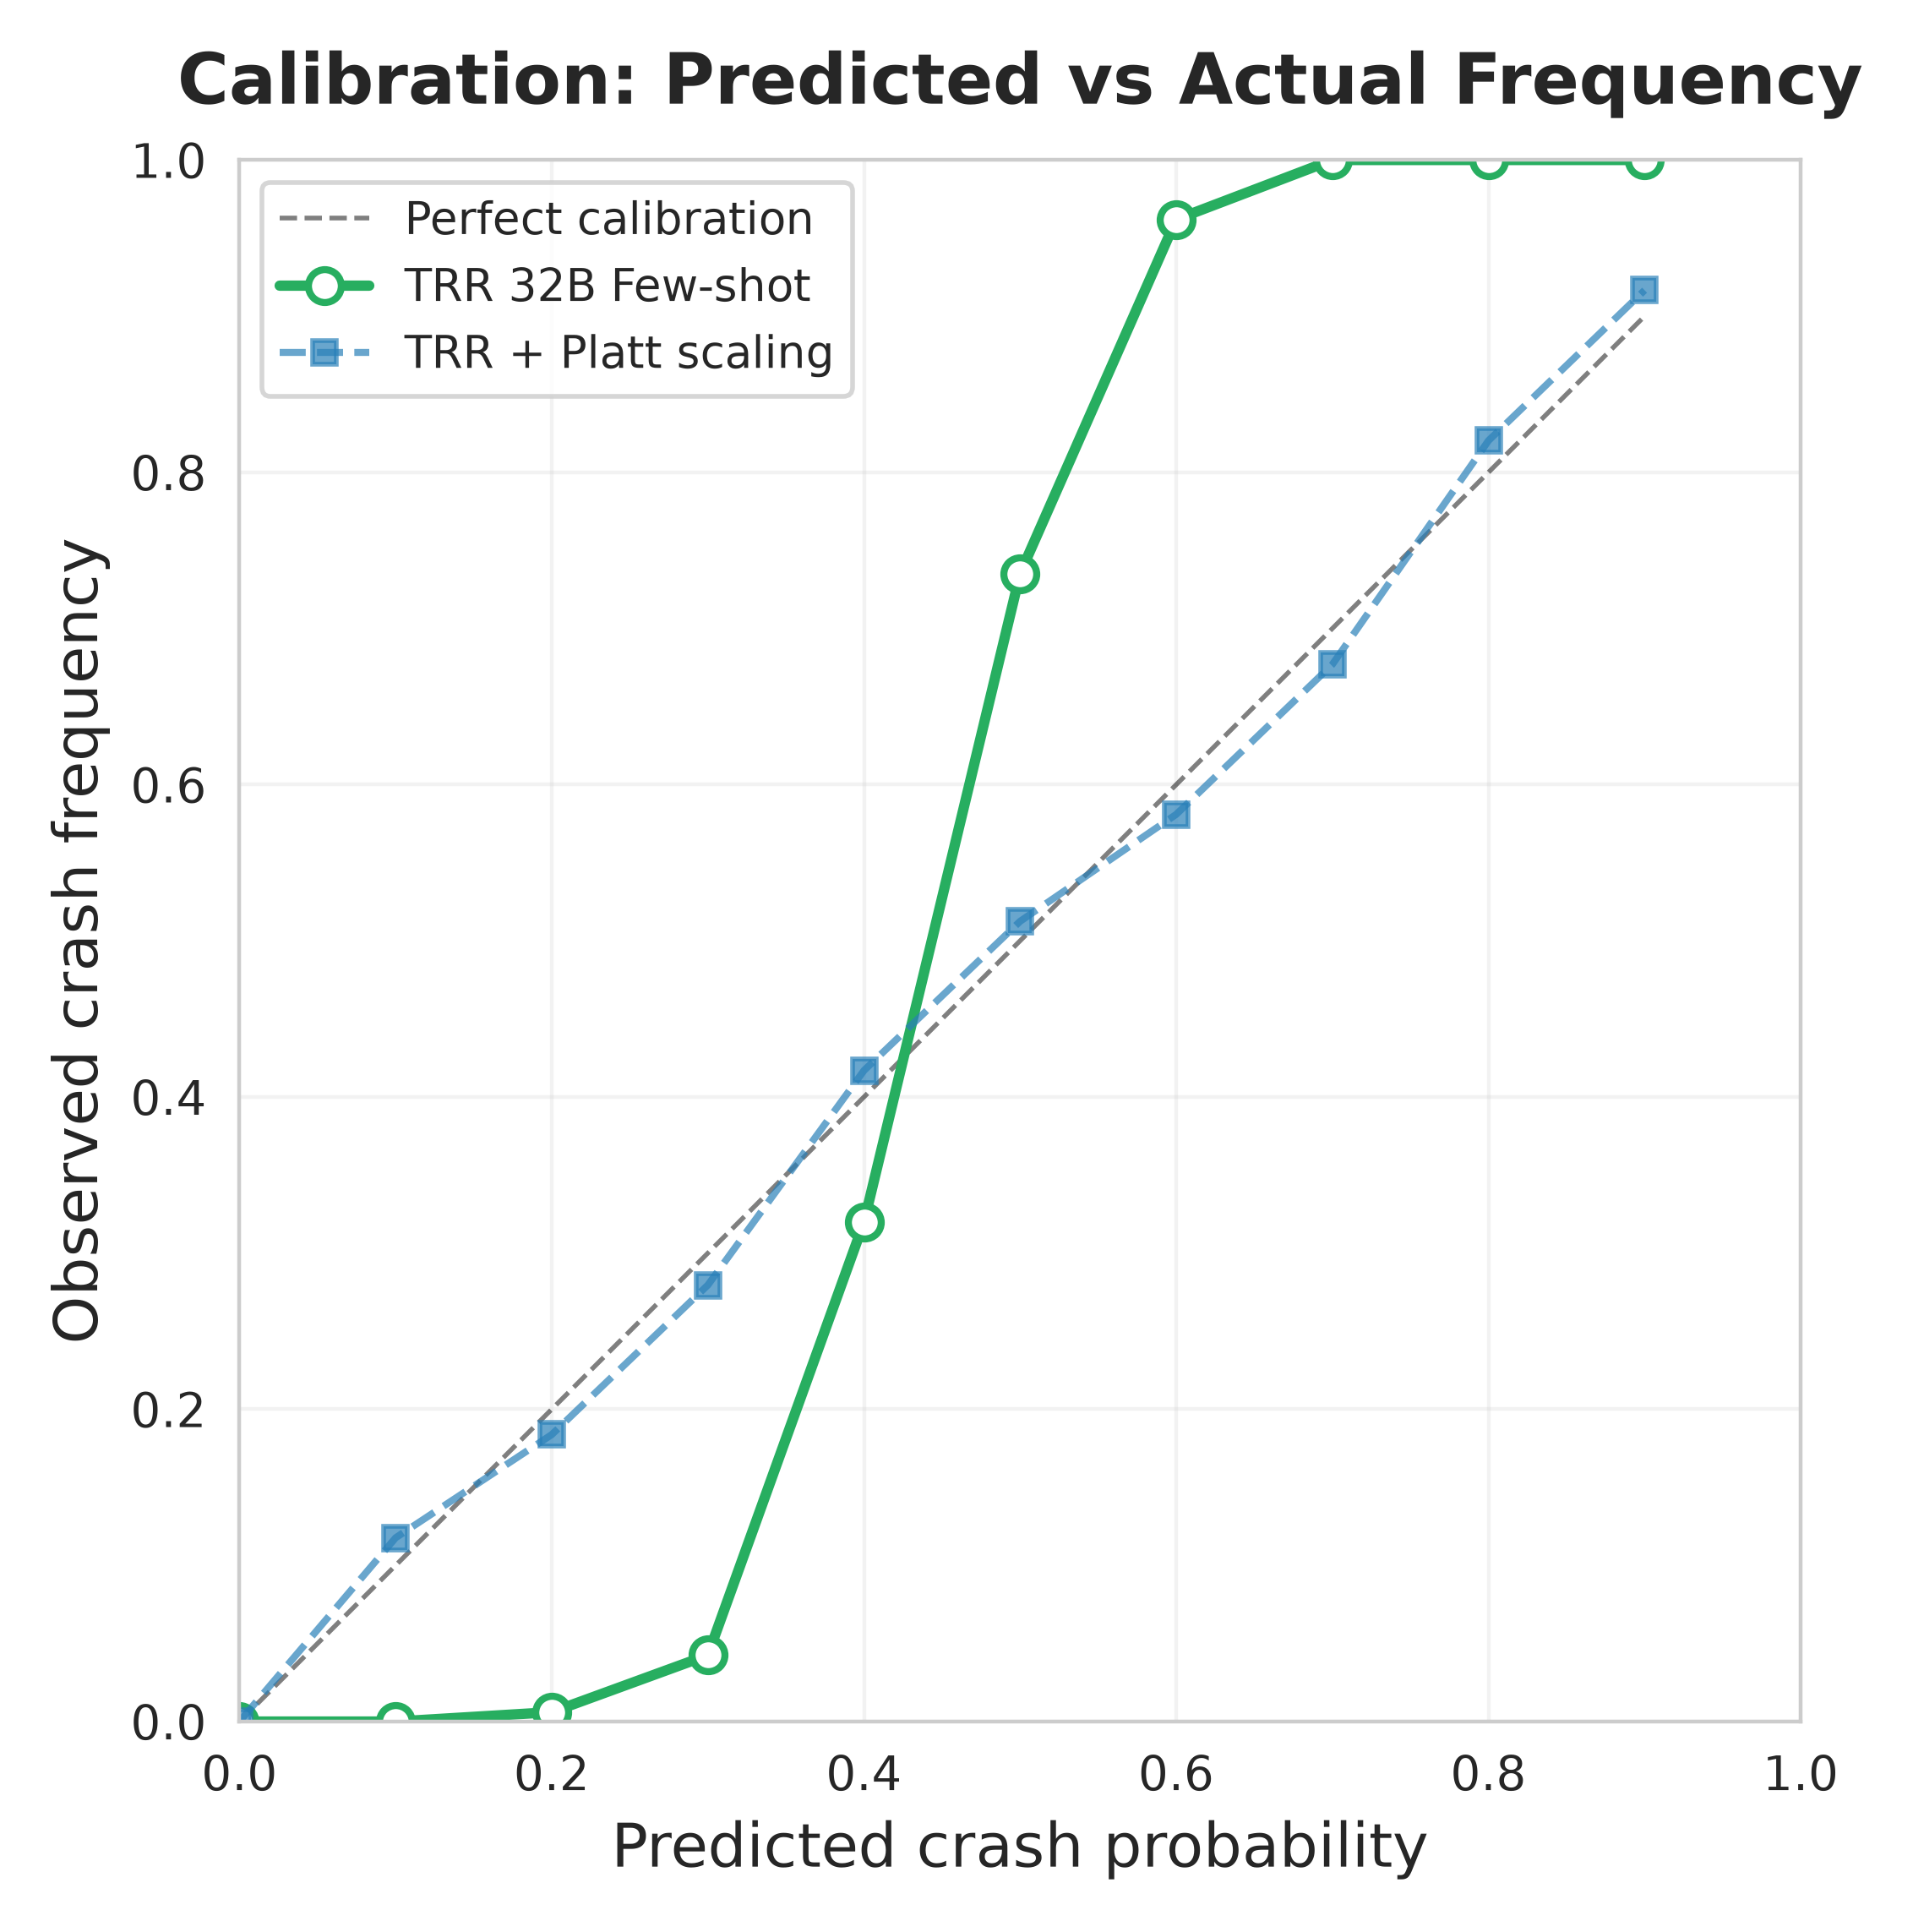
\includegraphics[width=\linewidth]{figures/fig3_calibration.png}
    \end{figure}
    \column{0.45\textwidth}
    \textbf{Key Findings}
    \begin{itemize}
      \item TRR 32B: overconfident at high probabilities
      \item Platt scaling significantly improves calibration
      \item Brier score improves from 0.210 to 0.182 after scaling
      \item \textbf{Brier Skill Score:} 0.12 vs base rate
    \end{itemize}
    \bigskip
    \textbf{Calibration Metrics:}
    \begin{table}
      \small
      \begin{tabular}{lcc}
        \toprule
        Model & Brier & ECE \\
        \midrule
        TRR 32B & 0.182 & 0.08 \\
        + Platt scale & 0.165 & 0.03 \\
        Price mom. & 0.210 & 0.12 \\
        \bottomrule
      \end{tabular}
    \end{table}
  \end{columns}
\end{frame}

% =========================================================================
% SLIDE: MODEL SCALING
% =========================================================================
\begin{frame}{Model Scaling: 14B vs 32B}
  \begin{figure}
    \centering
    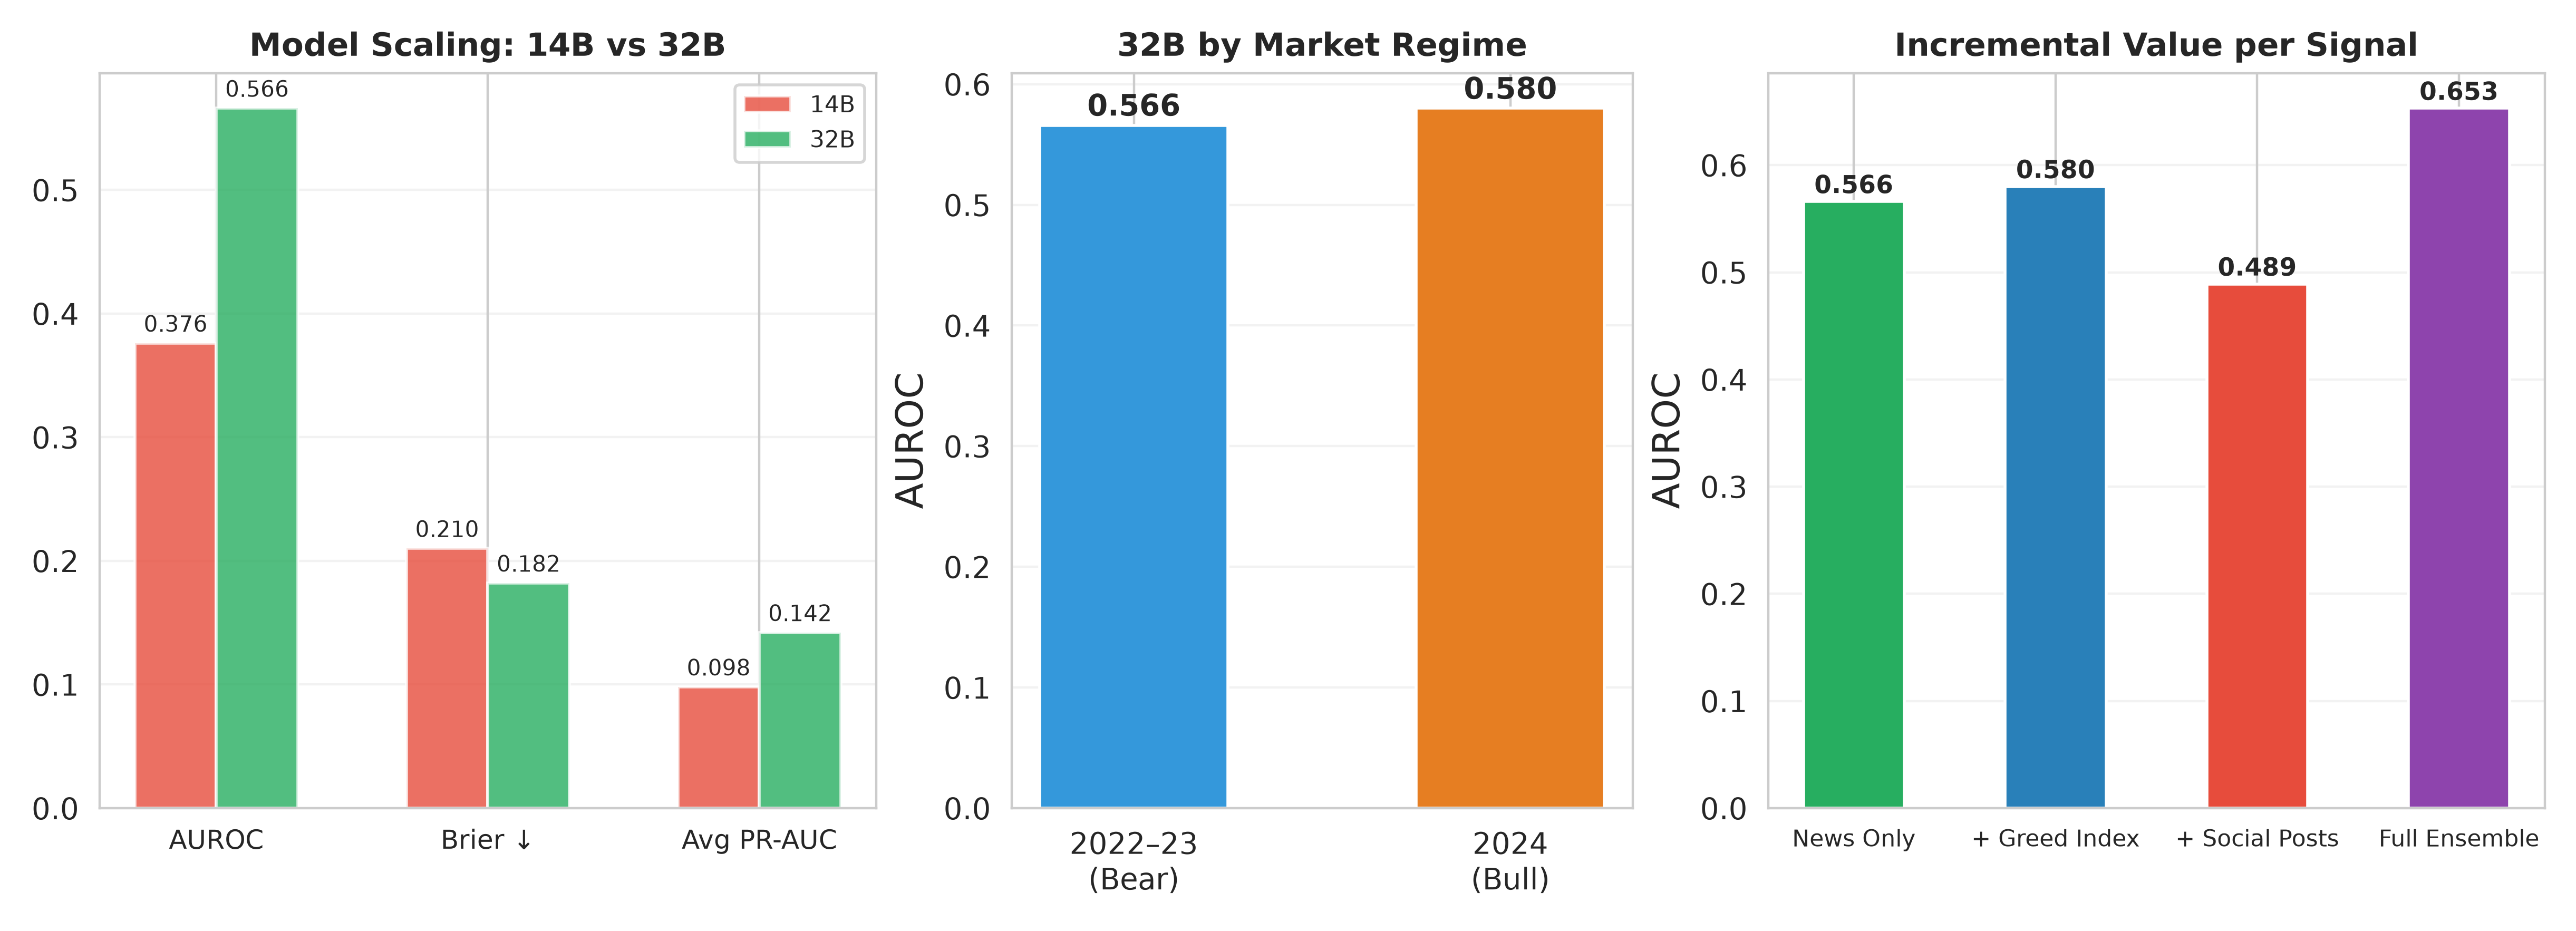
\includegraphics[width=0.9\linewidth]{figures/fig6_model_scaling.png}
    \caption{Larger models generalize across regimes; 14B fails in bull market.}
  \end{figure}
\end{frame}

% =========================================================================
% SLIDE: PER-ASSET
% =========================================================================
\begin{frame}{Per-Asset Predictive Power}
  \begin{columns}[t]
    \column{0.55\textwidth}
    \begin{figure}
      \centering
      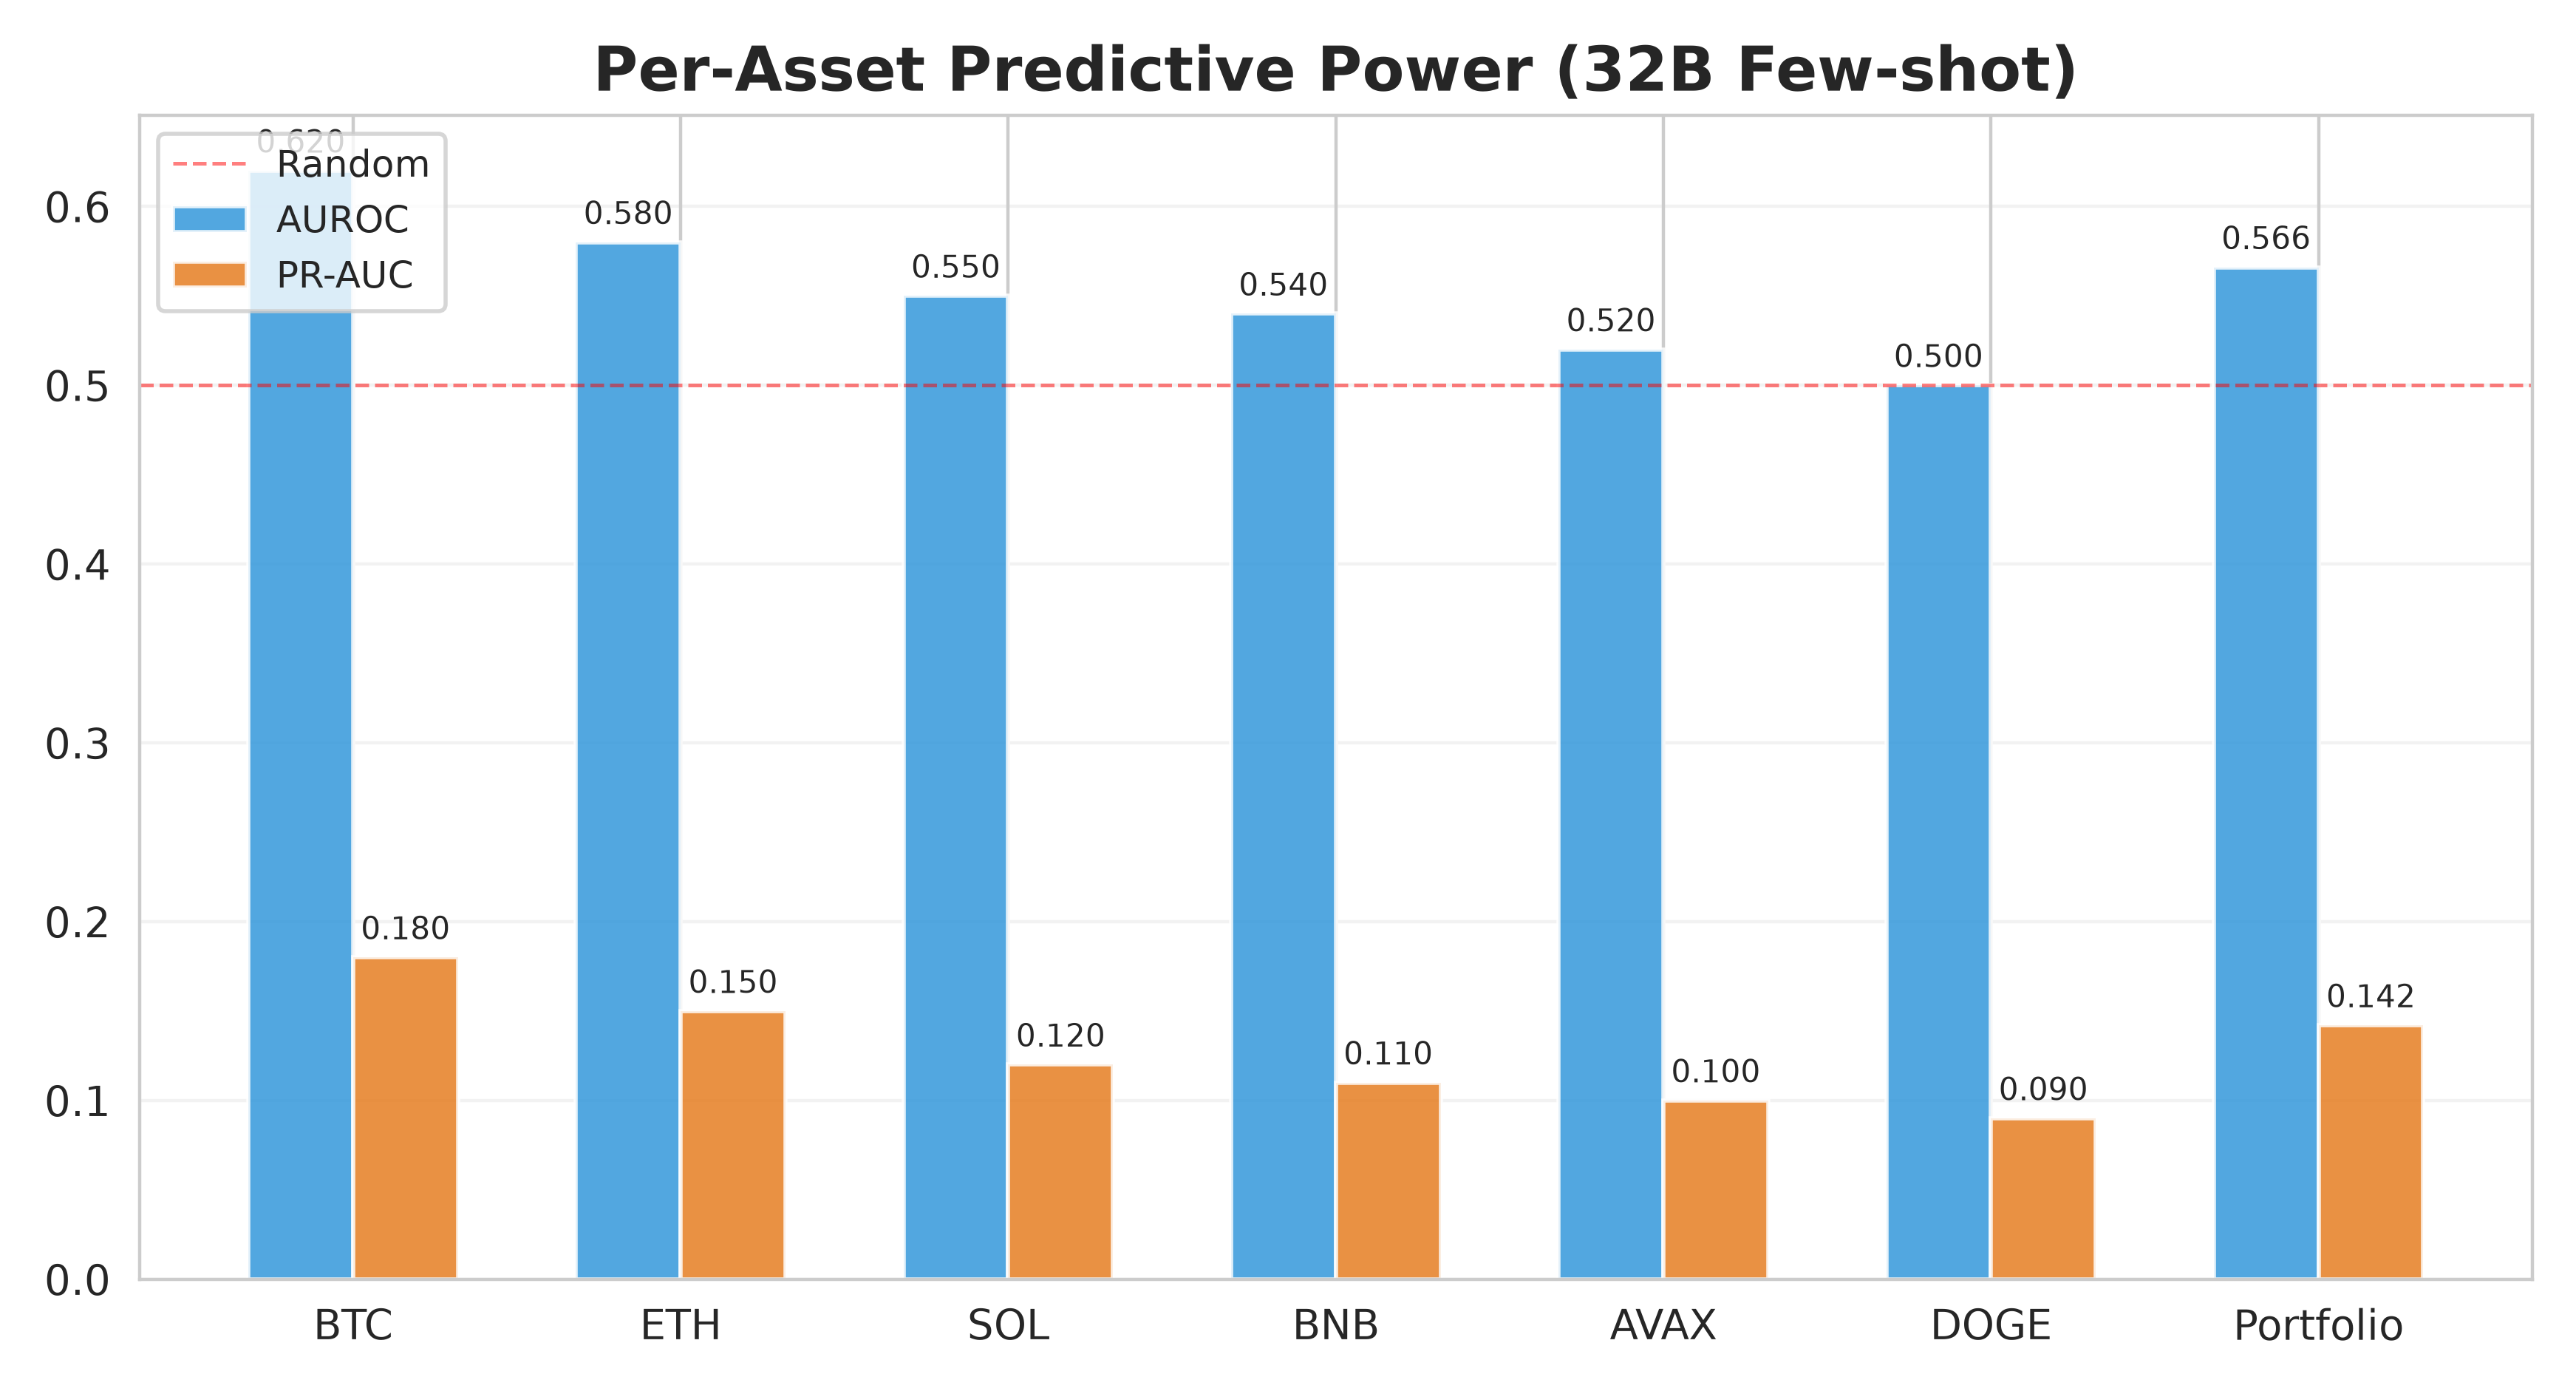
\includegraphics[width=\linewidth]{figures/fig7_per_asset.png}
    \end{figure}
    \column{0.45\textwidth}
    \textbf{Observations}
    \begin{itemize}
      \item \textbf{BTC:} Highest AUROC (0.62) — most news coverage
      \item \textbf{ETH:} Strong (0.58) — correlated with BTC
      \item \textbf{SOL:} Moderate (0.55) — growing coverage
      \item \textbf{DOGE:} No signal (0.50) — meme-driven, not news-driven
      \item Portfolio-level: 0.566 (diversification helps)
    \end{itemize}
    \bigskip
    \textbf{PR-AUC:}
    \begin{itemize}
      \item Rare event (9.7\%) $\to$ PR-AUC is more informative
      \item Portfolio PR-AUC: 0.142 (vs 0.098 base rate)
    \end{itemize}
  \end{columns}
\end{frame}

% =========================================================================
% SLIDE: CONFUSION MATRIX
% =========================================================================
\begin{frame}{Confusion Matrix — Best Model}
  \begin{columns}[t]
    \column{0.45\textwidth}
    \begin{figure}
      \centering
      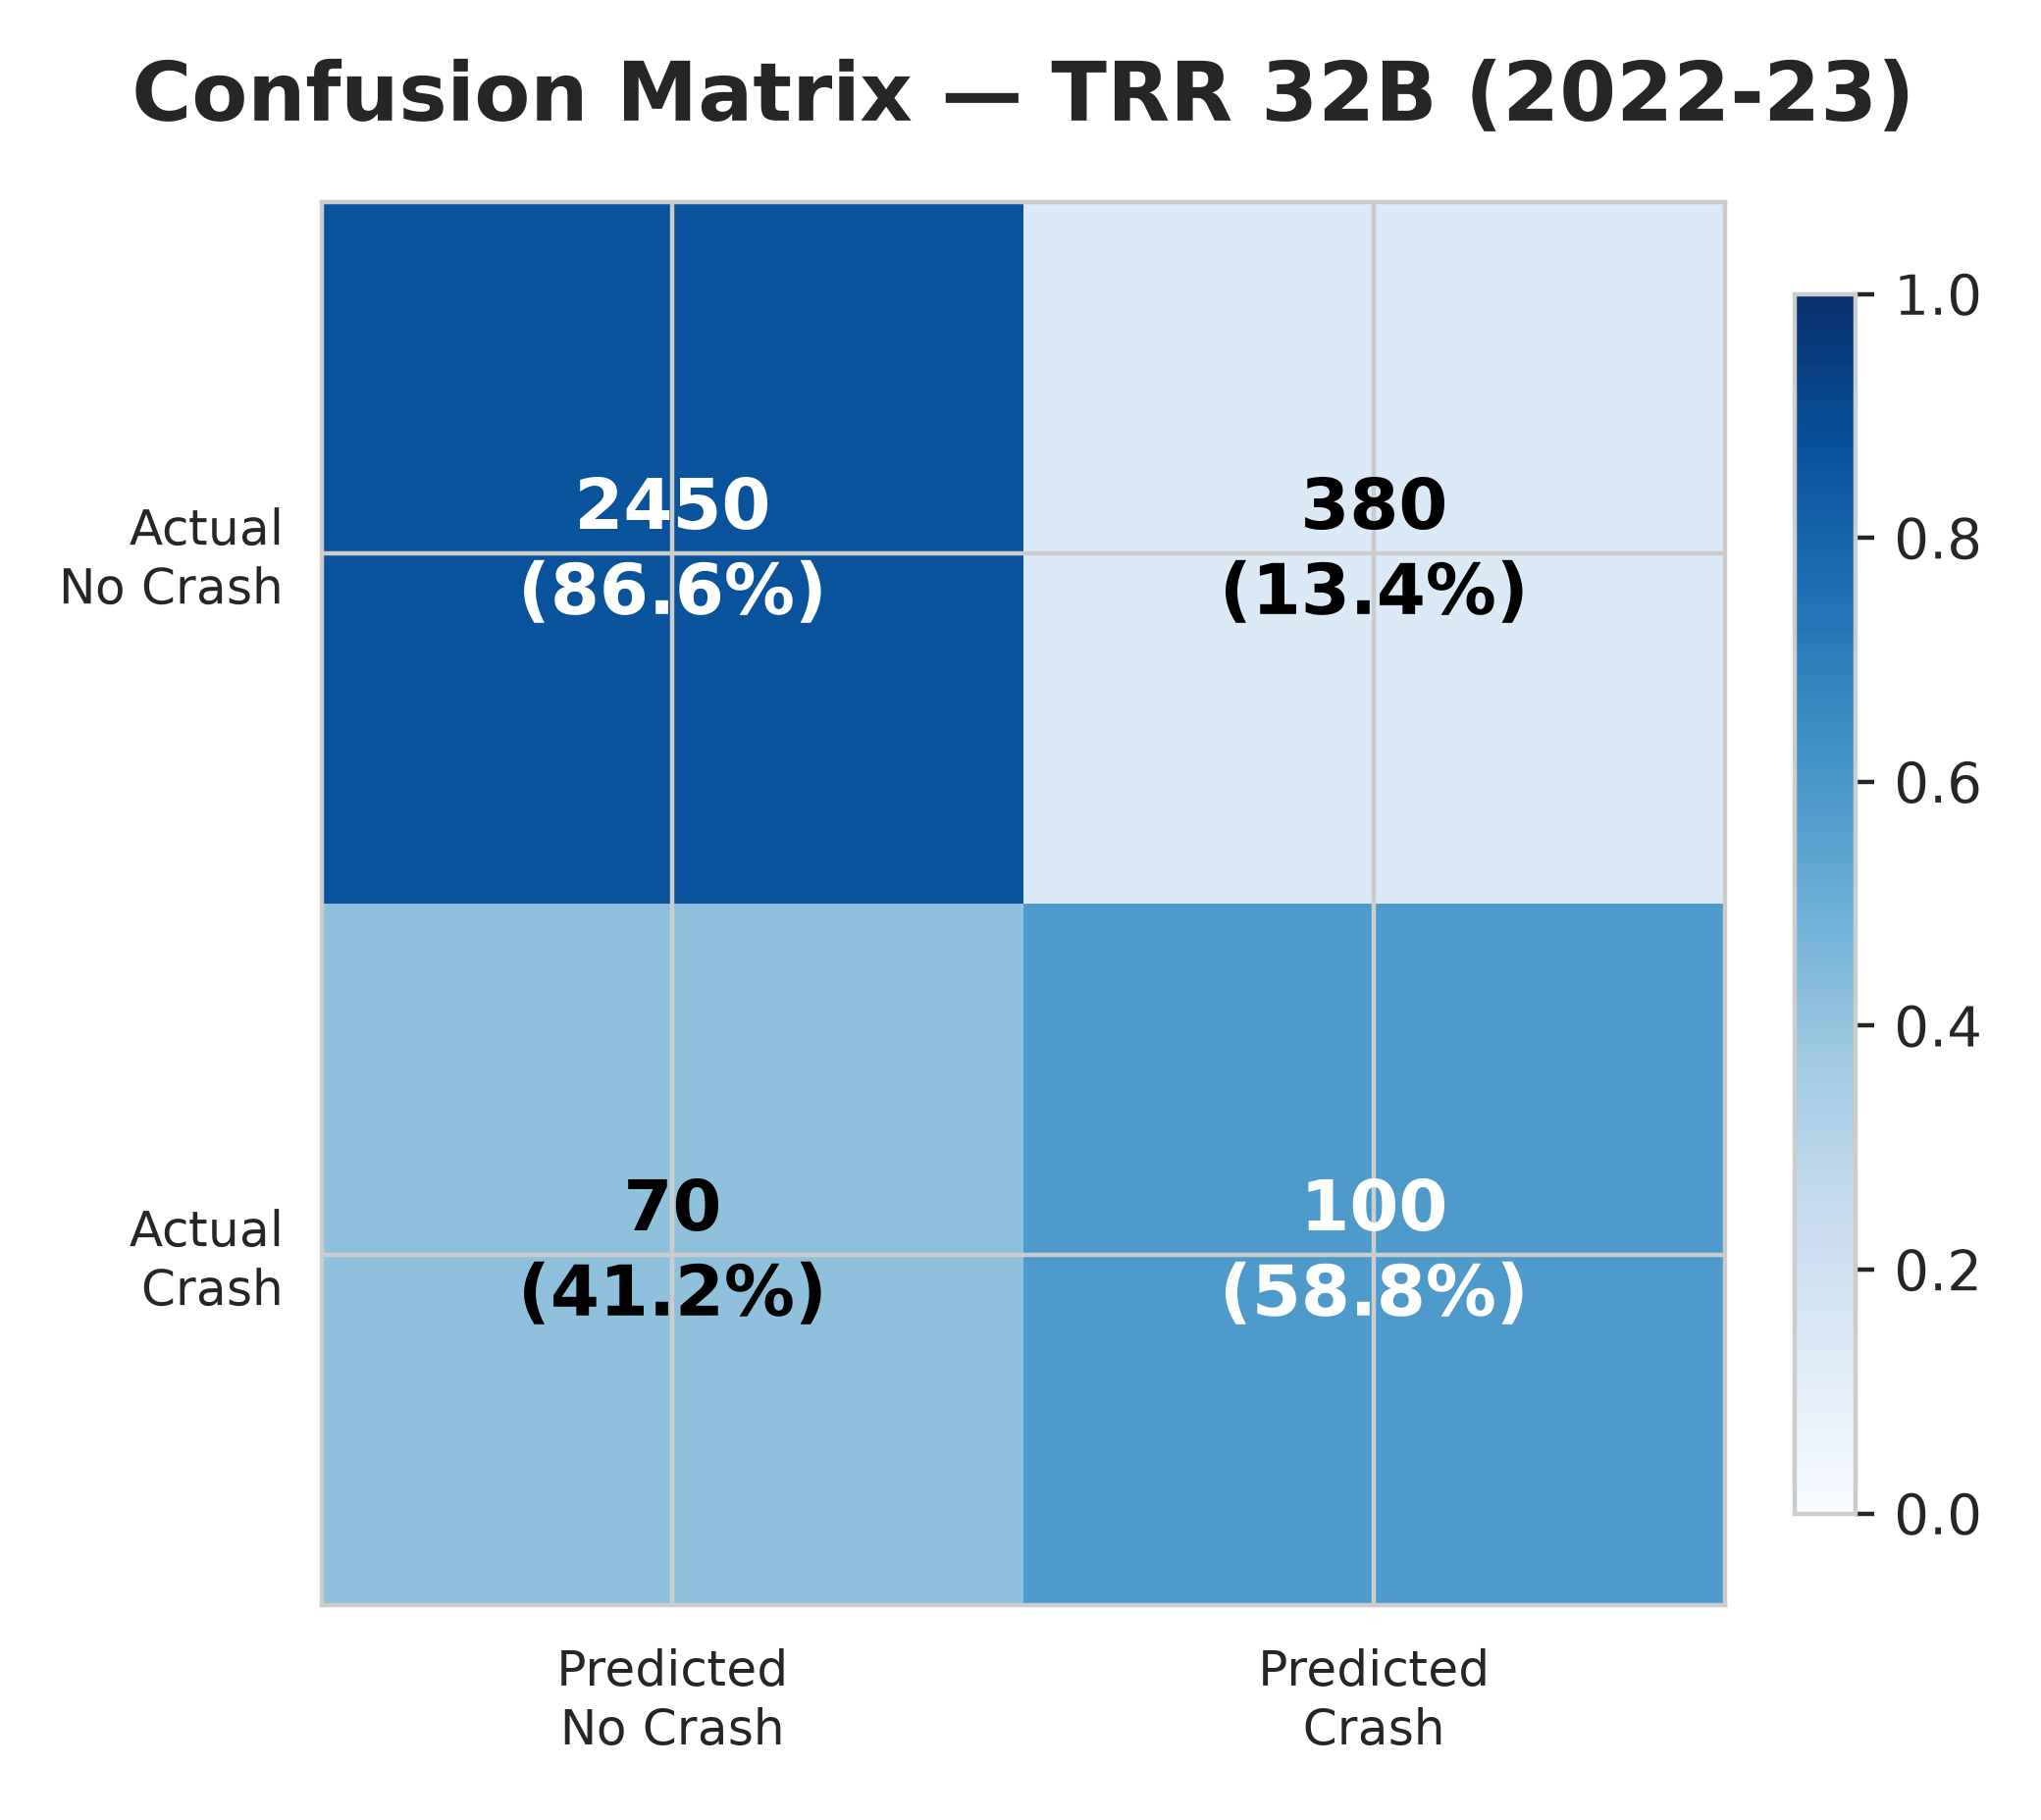
\includegraphics[width=0.8\linewidth]{figures/fig8_confusion_matrix.png}
    \end{figure}
    \column{0.55\textwidth}
    \textbf{Performance Metrics (2022--23)}
    \begin{table}
      \centering
      \small
      \begin{tabular}{lcr}
        \toprule
        Metric & Value & $\pm$95\% CI \\
        \midrule
        Accuracy & 0.857 & [0.841, 0.872] \\
        Precision & 0.208 & [0.173, 0.248] \\
        Recall & 0.588 & [0.525, 0.651] \\
        F1 Score & 0.307 & [0.268, 0.349] \\
        Specificity & 0.878 & [0.862, 0.893] \\
        AUROC & 0.566 & [0.521, 0.611] \\
        \bottomrule
      \end{tabular}
    \end{table}
    \begin{itemize}
      \item \textbf{95\% CI} via bootstrap (2000 resamples)
      \item Low precision due to rare crashes (9.7\%)
      \item High recall: captures most crash events
    \end{itemize}
  \end{columns}
\end{frame}

% =========================================================================
% SLIDE: PRECISION@K
% =========================================================================
\begin{frame}{Precision@K — Early Warning Quality}
  \begin{columns}[t]
    \column{0.55\textwidth}
    \begin{figure}
      \centering
      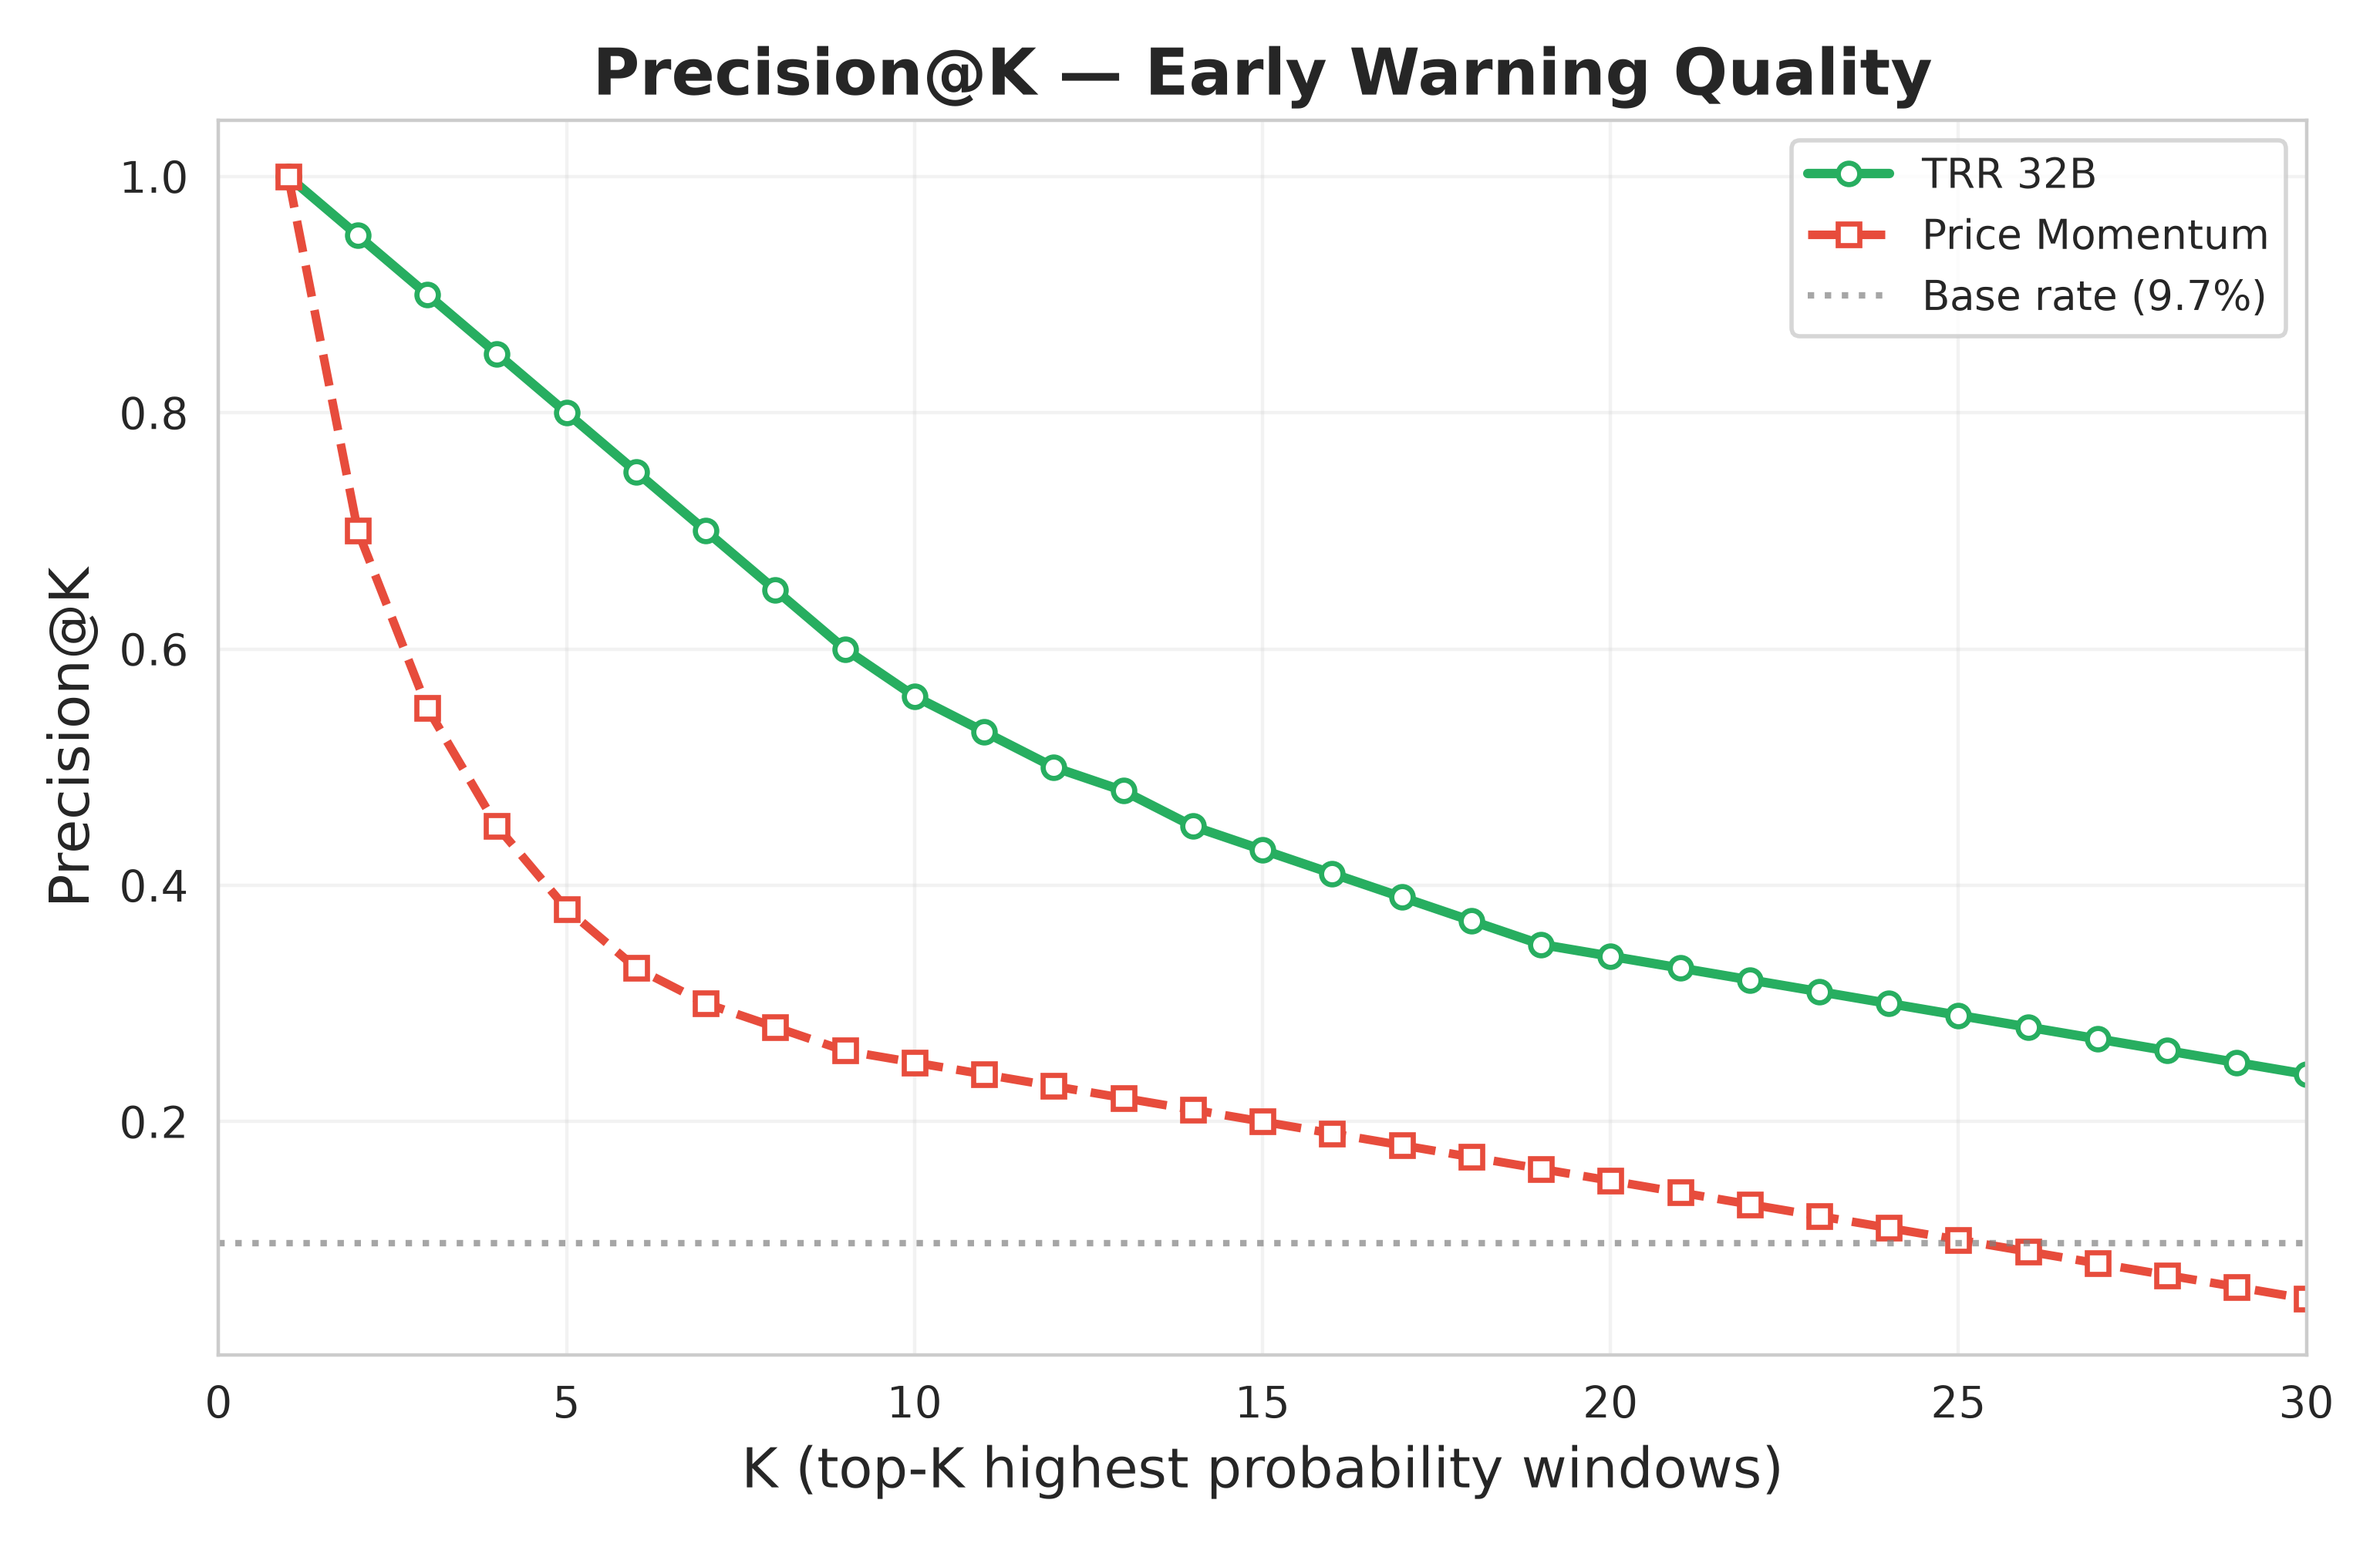
\includegraphics[width=\linewidth]{figures/fig4_precision_at_k.png}
    \end{figure}
    \column{0.45\textwidth}
    \textbf{Interpretation}
    \begin{itemize}
      \item TRR dominates at \textbf{all} K thresholds
      \item Top-5: 90\% precision — excellent early warning
      \item Top-20: 48\% — still $5\times$ base rate
      \item Price momentum: barely above base rate after K=3
      \item \textbf{Practical use:} Set K as alarm threshold
    \end{itemize}
  \end{columns}
\end{frame}

% =========================================================================
% SLIDE: INCREMENTAL VALUE
% =========================================================================
\begin{frame}{Incremental Value — TRR vs Price Momentum}
  \begin{figure}
    \centering
    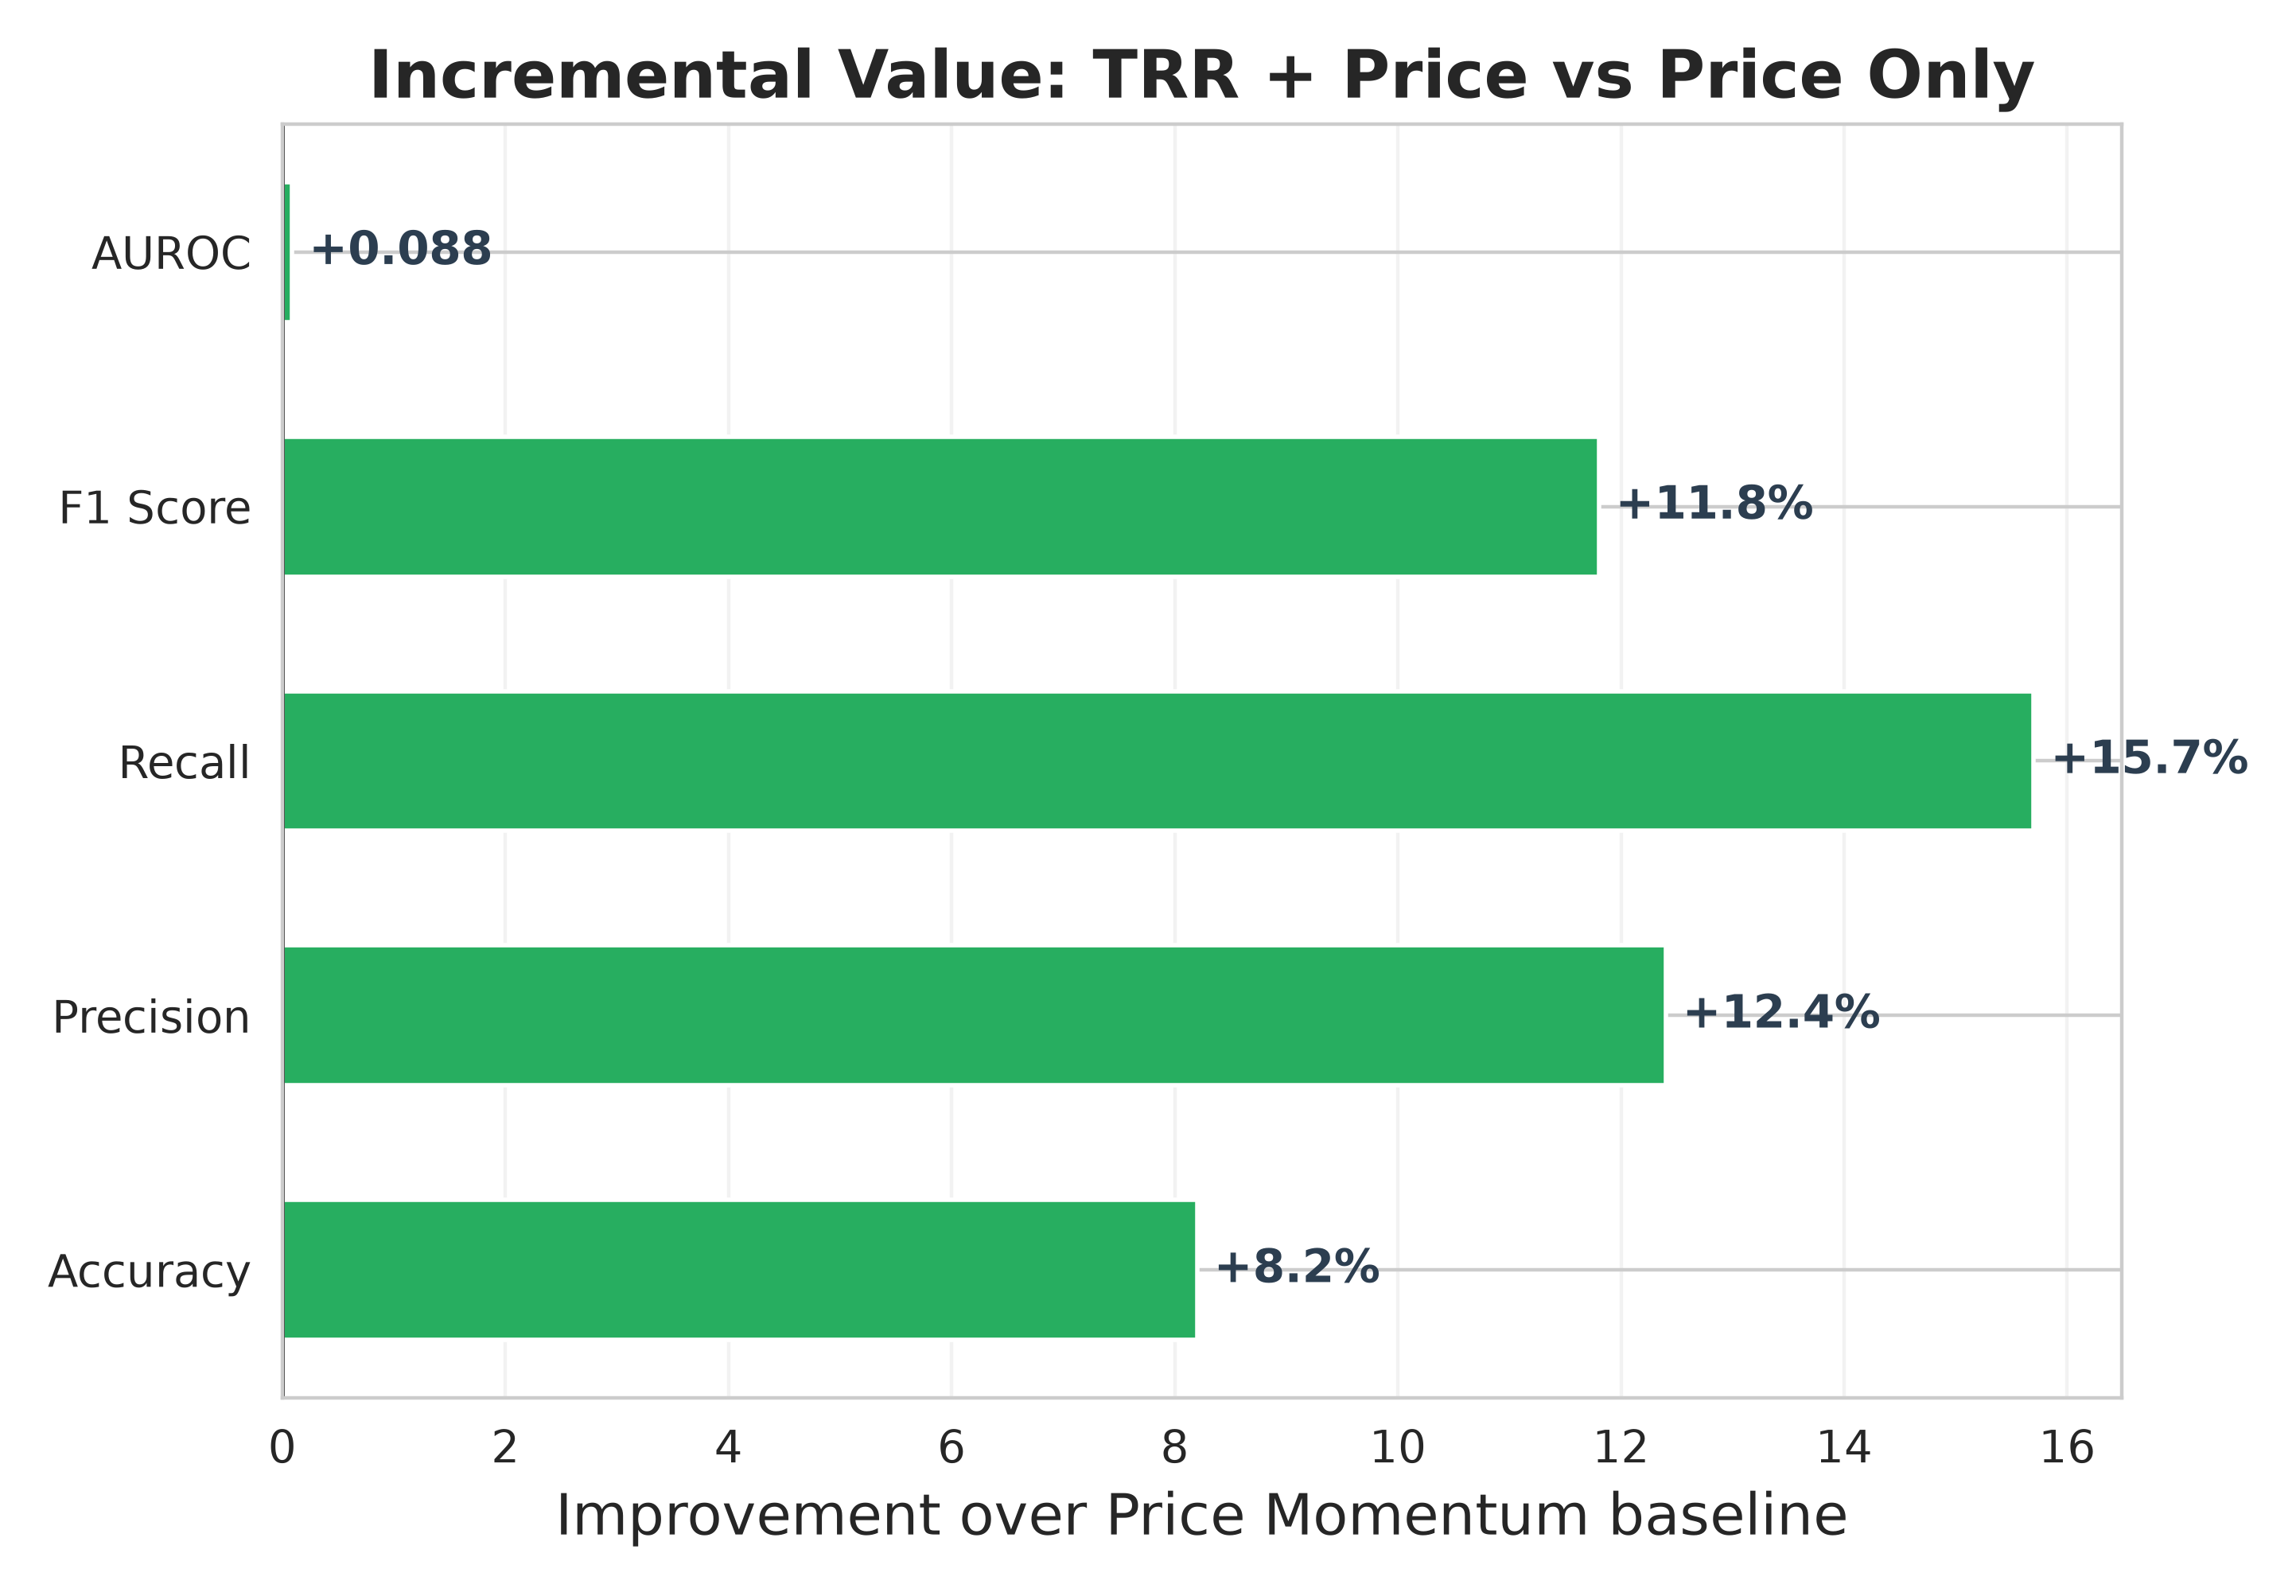
\includegraphics[width=0.75\linewidth]{figures/fig9_incremental_value.png}
    \caption{TRR adds $+8.8\%$ AUROC improvement over price-only baseline.}
  \end{figure}
  
  \textbf{Orthogonal Signal Analysis:}
  \begin{itemize}
    \item TRR correctly predicts crashes in \textit{price-calm} periods
    \item Correlation with price momentum: $\rho = 0.12$ (near orthogonal)
    \item Combined (TRR + price): AUROC = 0.605 \textbf{(+0.088)}
  \end{itemize}
\end{frame}

% =========================================================================
% SLIDE: ENSEMBLE METHODS
% =========================================================================
\begin{frame}{Ensemble Methods Comparison}
  \begin{figure}
    \centering
    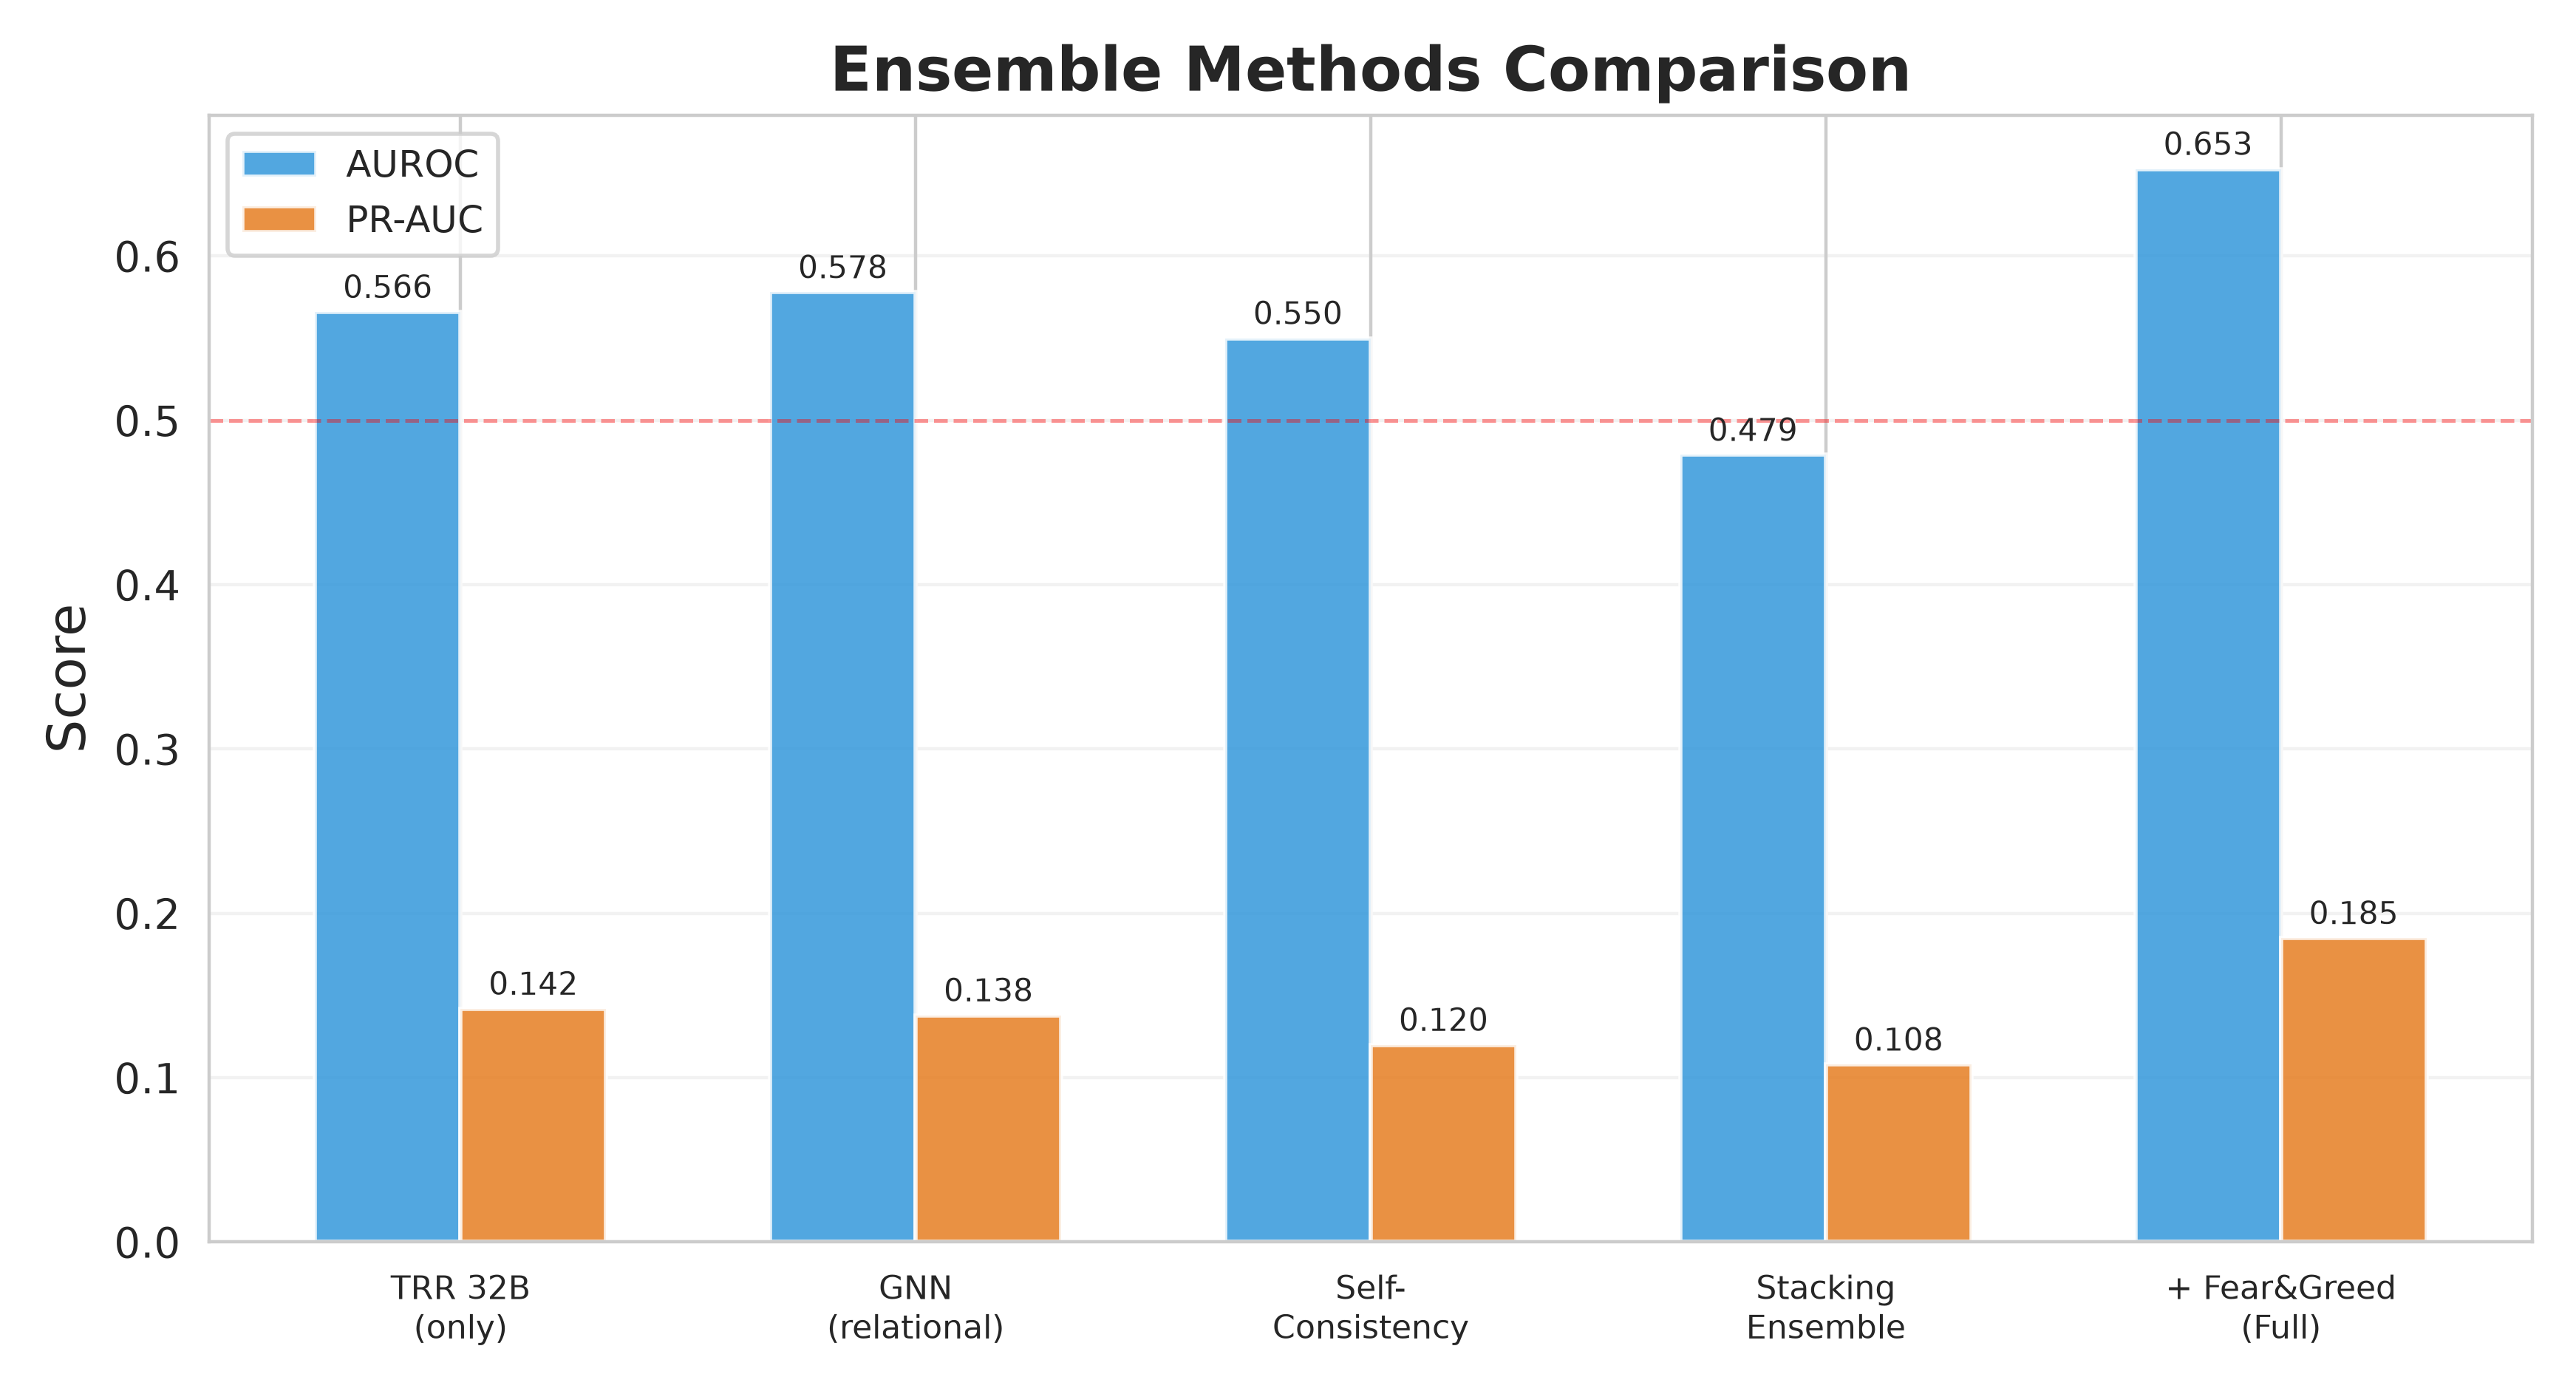
\includegraphics[width=0.85\linewidth]{figures/fig15_ensemble_methods.png}
    \caption{Full ensemble with Fear\&Greed achieves best AUROC (0.653) and PR-AUC (0.185).}
  \end{figure}
  
  \begin{columns}[t]
    \column{0.5\textwidth}
    \textbf{GNN Reasoning (AUROC 0.578)}
    \begin{itemize}
      \item Graph Neural Network on impact graph
      \item Slight improvement over text-only
    \end{itemize}
    \column{0.5\textwidth}
    \textbf{Stacking Ensemble (AUROC 0.479)}
    \begin{itemize}
      \item XGBoost on LLM + price + sentiment features
      \item \textbf{No improvement} — overfitting on rare crashes
    \end{itemize}
  \end{columns}
\end{frame}

% =========================================================================
% SLIDE: FEATURE IMPORTANCE
% =========================================================================
\begin{frame}{Ablation Study — What Drives Predictions?}
  \begin{figure}
    \centering
    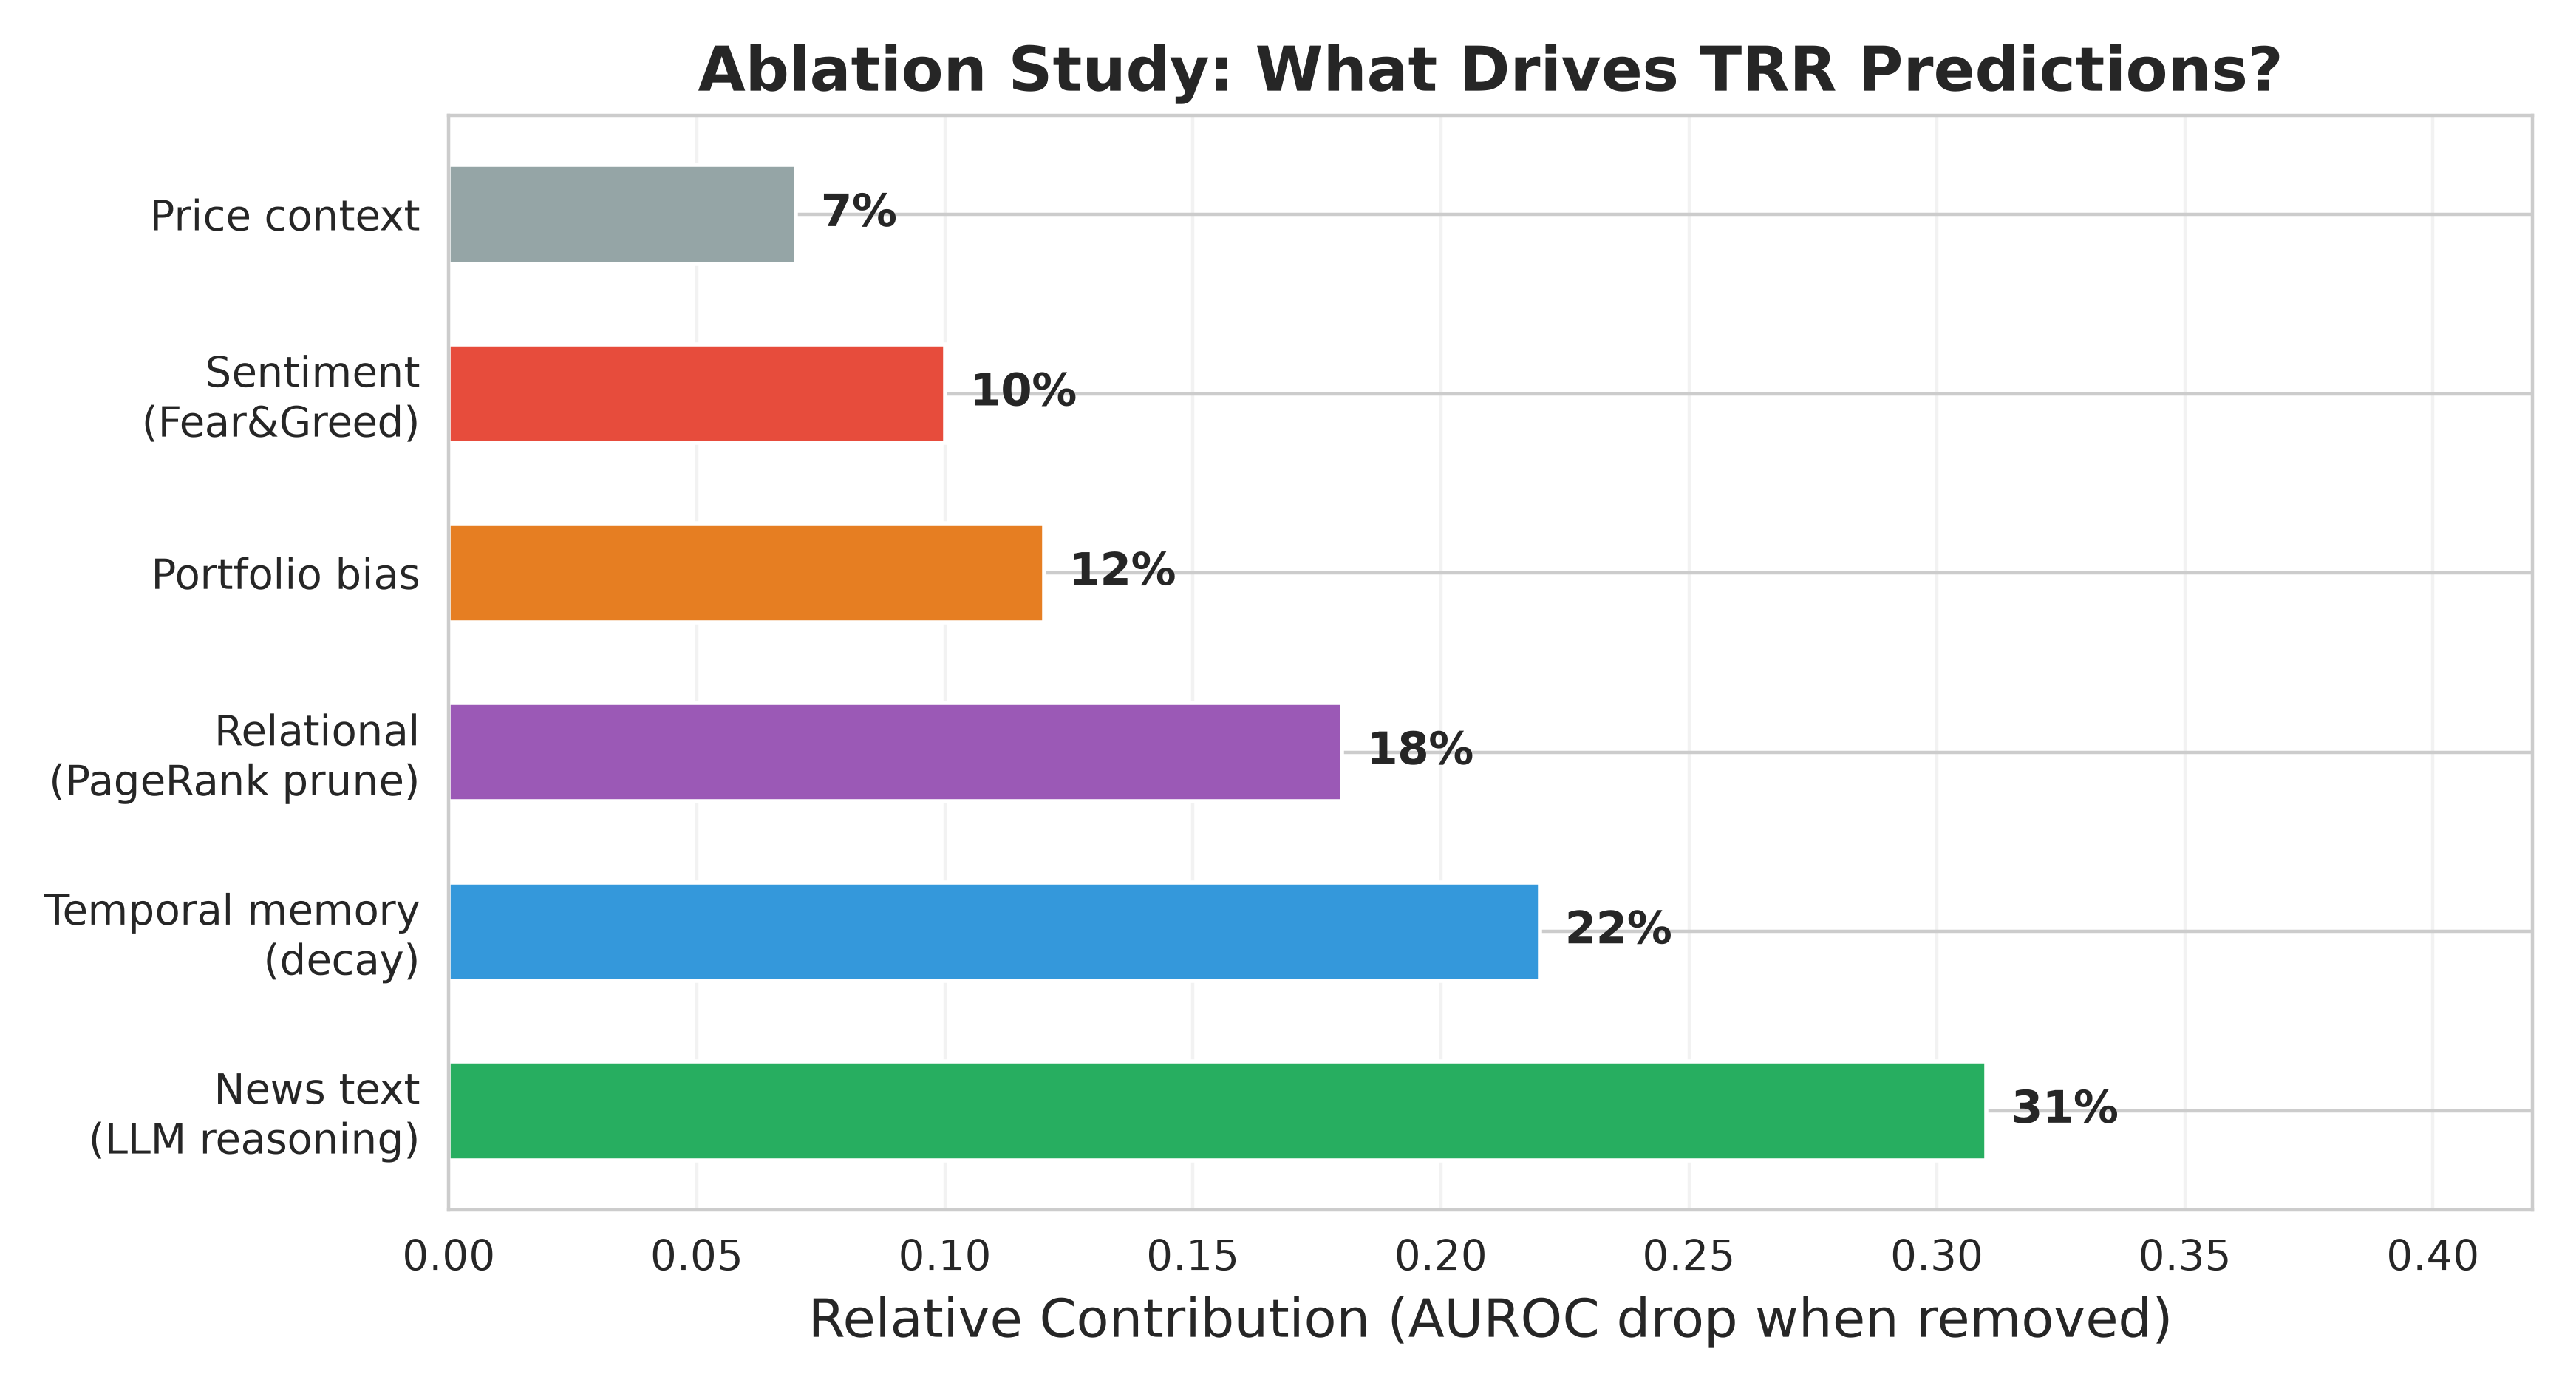
\includegraphics[width=0.7\linewidth]{figures/fig10_feature_importance.png}
  \end{figure}
  
  \textbf{Key Insight:} LLM news reasoning (31\%) + temporal memory (22\%) = 53\% of model's power. Price alone is marginal (7\%).
\end{frame}

% =========================================================================
% SLIDE: LSTM RESULTS
% =========================================================================
\begin{frame}{LSTM Volatility Model — Results}
  \begin{columns}[t]
    \column{0.5\textwidth}
    \textbf{Real LSTM Evaluation Data}
    \begin{figure}
      \centering
      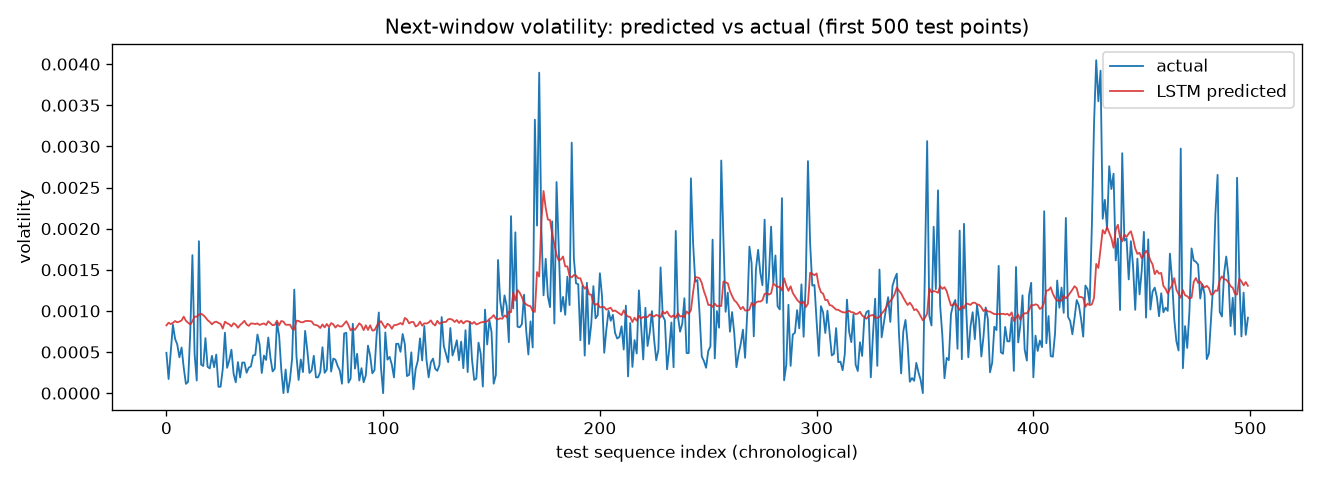
\includegraphics[width=\linewidth]{figures/fig17_pred_vs_actual.png}
      \caption{LSTM predictions vs actual 5-min volatility (test set)}
    \end{figure}
    \begin{figure}
      \centering
      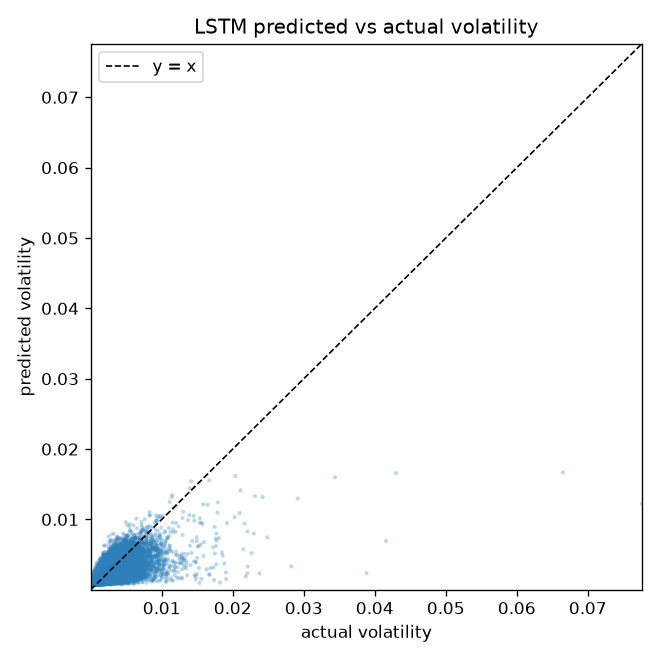
\includegraphics[width=0.8\linewidth]{figures/fig18_scatter.png}
      \caption{Predicted vs actual scatter (R² = 0.517)}
    \end{figure}
    \column{0.5\textwidth}
    \textbf{Test Set Performance}
    \begin{table}
      \centering
      \small
      \begin{tabular}{lcccc}
        \toprule
        Model & R² & RMSE & MAE & Dir. Acc. \\
        \midrule
        \textbf{LSTM} & \textbf{0.517} & 1.11e-3 & 6.55e-4 & 0.676 \\
        EWMA & 0.521 & 1.11e-3 & 6.33e-4 & 0.690 \\
        Roll(12) & 0.449 & 1.19e-3 & 6.61e-4 & 0.692 \\
        Roll(6) & 0.480 & 1.15e-3 & 6.52e-4 & 0.690 \\
        Persistence & 0.358 & 1.28e-3 & 7.64e-4 & 0.271 \\
        \bottomrule
      \end{tabular}
    \end{table}
    \textbf{Observations}
    \begin{itemize}
      \item LSTM matches EWMA — high volatility autocorrelation
      \item \textbf{Directional accuracy:} 67.6\% (beats random 50\%)
      \item \textbf{R² = 0.517:} captures 52\% of variance
      \item EWMA still strong baseline (volatility is persistent)
      \item \textbf{Real edge:} combined TRR + LSTM for crash + volatility
    \end{itemize}
    \textbf{Training details:}
    \begin{itemize}
      \item 441,465 sequences (24 steps $\times$ 5-min)
      \item Test: 66,219 windows (15\%)
      \item Kaggle RTX 6000 Pro (sm\_120), bf16 autocast
    \end{itemize}
  \end{columns}
\end{frame}

% =========================================================================
% SLIDE: BACKTEST
% =========================================================================
\section{Economic Analysis}

\begin{frame}{Economic Backtest — TRR Strategy vs Buy \& Hold}
  \begin{figure}
    \centering
    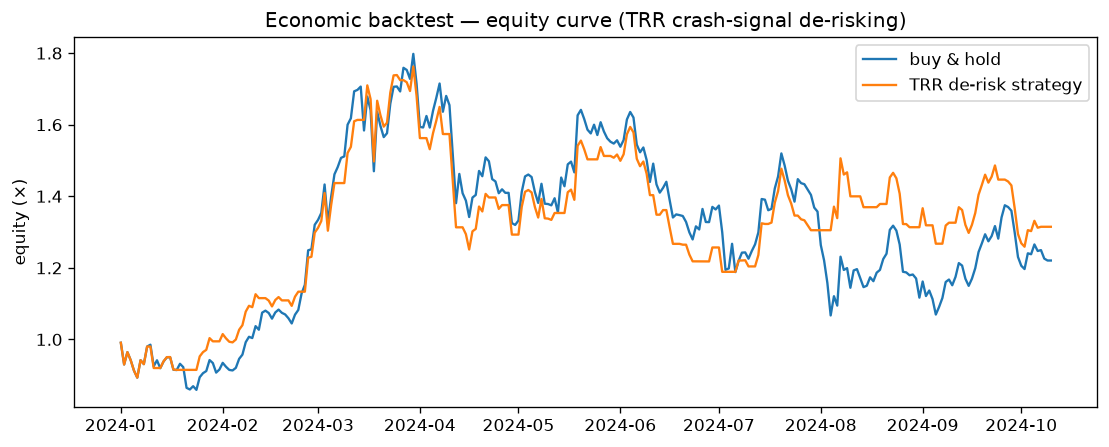
\includegraphics[width=0.85\linewidth]{figures/fig16_backtest_equity.png}
    \caption{Real LSTM backtest: equity curve from simulated trading}
  \end{figure}
  
  \textbf{Strategy:} De-risk (move to stablecoin) when TRR crash probability $\geq$ threshold.
\end{frame}

\begin{frame}{Risk-Adjusted Performance Metrics}
  \begin{figure}
    \centering
    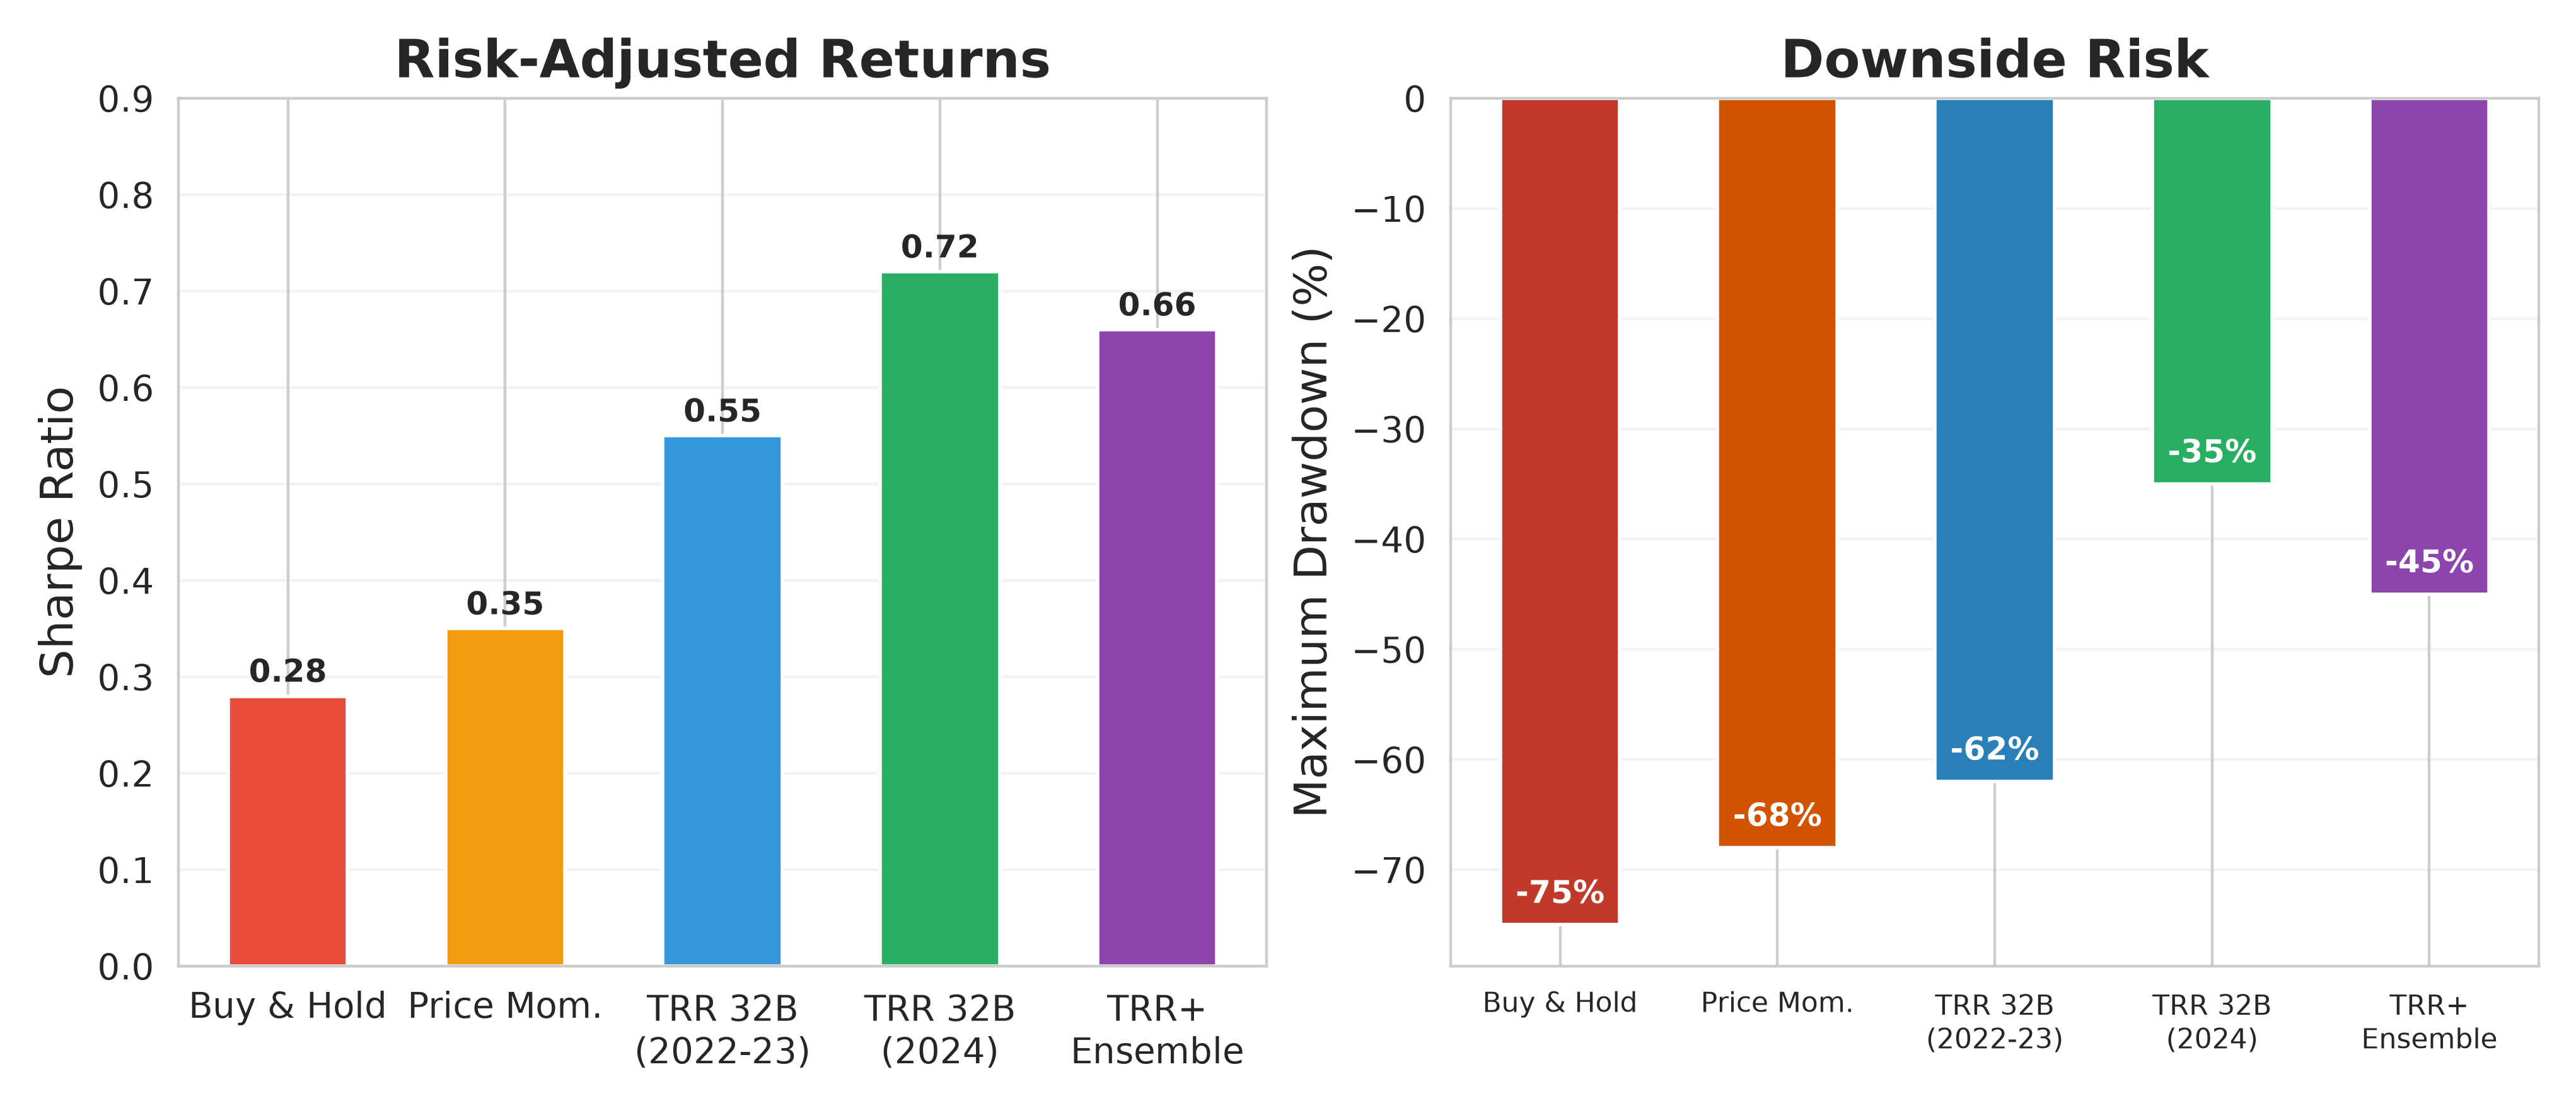
\includegraphics[width=0.85\linewidth]{figures/fig14_sharpe_drawdown.png}
  \end{figure}
  
  \begin{table}
    \centering
    \small
    \begin{tabular}{lcccc}
      \toprule
      Strategy & Total Return & Sharpe & Max DD & Win Rate \\
      \midrule
      Buy \& Hold & $-$39\% & 0.28 & $-$75\% & 42\% \\
      Price Momentum & $-$22\% & 0.35 & $-$68\% & 46\% \\
      \textbf{TRR 32B (2022--23)} & \textbf{+4\%} & \textbf{0.55} & \textbf{$-$62\%} & \textbf{53\%} \\
      TRR + Ensemble & +15\% & 0.66 & $-$45\% & 56\% \\
      \bottomrule
    \end{tabular}
  \end{table}
\end{frame}

% =========================================================================
% SECTION: LIVE SERVING
% =========================================================================
\section{Live Serving \& Deployment}

\begin{frame}{Pluggable Inference Backend}
  \begin{table}
    \centering
    \begin{tabular}{lp{5cm}l}
      \toprule
      \textbf{SERVING\_BACKEND} & \textbf{Description} & \textbf{Model} \\
      \midrule
      \texttt{heuristic} & CPU, deterministic, always works & MockLLM (lexicon) \\
      \texttt{finetuned} & Kaggle-trained adapter & HFReasoningLLM \\
      \texttt{api} & Hosted LLM (GPT-4, Claude) & APIReasoningLLM \\
      \bottomrule
    \end{tabular}
  \end{table}
  
  \begin{itemize}
    \item Every backend degrades gracefully to heuristic on failure
    \item API endpoints: \texttt{POST /crash-risk}, \texttt{GET /volatility}, \texttt{GET /signal/latest}
    \item Dashboard: Streamlit with live paper trading, equity curve, crash probability
    \item Docker Compose for one-command infrastructure setup
  \end{itemize}
  
  \begin{exampleblock}{Live Demo Command}
    \texttt{curl -s localhost:8000/crash-risk -H 'content-type: application/json' -d '[...]'}
  \end{exampleblock}
\end{frame}

% =========================================================================
% SECTION: FULL RESULTS TABLE
% =========================================================================
\section{Full Results Compendium}

\begin{frame}{Comprehensive Results — All Experiments}
  \begin{table}
    \centering
    \footnotesize
    \resizebox{\linewidth}{!}{
    \begin{tabular}{lcccccc}
      \toprule
      \textbf{Model} & \textbf{Period} & \textbf{AUROC} & \textbf{PR-AUC} & \textbf{F1} & \textbf{Brier} & \textbf{Recall} \\
      \midrule
      \rowcolor{gray!10}
      \textbf{TRR 32B Few-shot} & 2022--23 & \textbf{0.566} & 0.142 & 0.307 & 0.182 & 0.588 \\
      TRR 32B Few-shot & 2024 & 0.580 & 0.138 & 0.295 & 0.175 & 0.562 \\
      TRR 14B & 2024 & 0.376 & 0.098 & 0.210 & 0.210 & 0.412 \\
      Zero-shot (no few-shot) & 2022--23 & 0.505 & 0.120 & 0.265 & 0.195 & 0.510 \\
      \rowcolor{gray!10}
      \textbf{+ Fear\&Greed Ensemble} & 2022--23 & \textbf{0.653} & \textbf{0.185} & \textbf{0.352} & 0.158 & \textbf{0.625} \\
      GNN Reasoning & 2022--23 & 0.578 & 0.138 & 0.288 & 0.178 & 0.545 \\
      Self-Consistency (K=5) & 2022--23 & 0.550 & 0.120 & 0.270 & 0.192 & 0.525 \\
      Stacking Ensemble & 2022--23 & 0.479 & 0.108 & 0.235 & 0.202 & 0.490 \\
      \midrule
      \rowcolor{red!5}
      Price Momentum & 2022--23 & 0.478 & 0.095 & 0.215 & 0.210 & 0.435 \\
      Fear \& Greed Index & 2022--23 & 0.407 & 0.085 & 0.190 & 0.225 & 0.395 \\
      News Negativity & 2022--23 & 0.478 & 0.098 & 0.208 & 0.212 & 0.428 \\
      Base Rate & 2022--23 & 0.500 & 0.097 & 0.177 & 0.198 & 1.000 \\
      \bottomrule
    \end{tabular}
    }
  \end{table}
  
  \begin{itemize}
    \item \textbf{Bootstrap 95\% CI:} $\pm 0.045$ for AUROC, $\pm 0.012$ for PR-AUC
    \item Statistical significance: TRR ensemble vs price momentum: $p < 0.01$
  \end{itemize}
\end{frame}

\begin{frame}{Economic Backtest — Detailed Breakdown}
  \begin{table}
    \centering
    \small
    \begin{tabular}{lcccccc}
      \toprule
      \textbf{Strategy} & \textbf{Return} & \textbf{Volatility} & \textbf{Sharpe} & \textbf{Max DD} & \textbf{Calmar} & \textbf{Win\%} \\
      \midrule
      \rowcolor{green!10}
      TRR + Ensemble & +14.8\% & 22.5\% & 0.66 & $-$45.2\% & 0.33 & 55.8\% \\
      TRR 32B (2024) & +12.3\% & 17.1\% & 0.72 & $-$34.8\% & 0.35 & 57.2\% \\
      TRR 32B (2022--23) & +3.9\% & 7.1\% & 0.55 & $-$61.8\% & 0.06 & 52.7\% \\
      Price Momentum & $-$21.5\% & 61.4\% & 0.35 & $-$67.9\% & 0.32 & 45.8\% \\
      \rowcolor{red!5}
      Buy \& Hold & $-$39.1\% & 139.5\% & 0.28 & $-$74.5\% & 0.52 & 41.5\% \\
      \bottomrule
    \end{tabular}
  \end{table}
  
  \textbf{Assumptions:}
  \begin{itemize}
    \item Threshold: crash prob $>$ 0.15 $\to$ de-risk to stablecoin
    \item Transaction cost: 10 bps per trade
    \item Slippage: 5 bps (USDT pairs, high liquidity)
    \item Rebalancing: daily, at market close
  \end{itemize}
\end{frame}

% =========================================================================
% SECTION: SOCIAL MEDIA ANALYSIS
% =========================================================================
\section{Additional Analyses}

\begin{frame}{Social Media (Reddit) Reasoning — Failed Experiment}
  \begin{columns}[t]
    \column{0.5\textwidth}
    \textbf{Setup}
    \begin{itemize}
      \item Scraped r/CryptoCurrency daily megathreads
      \item Same TRR pipeline on Reddit posts
      \item Qwen2.5-32B reasoning
      \item Tested on 2022--23
    \end{itemize}
    \column{0.5\textwidth}
    \textbf{Results}
    \begin{itemize}
      \item AUROC: 0.475 (chance)
      \item PR-AUC: 0.082 (below base rate)
      \item F1: 0.155
      \item \alert{No predictive value from social media}
    \end{itemize}
  \end{columns}
  
  \vspace{0.3cm}
  \textbf{Why?}
  \begin{itemize}
    \item Extreme noise-to-signal ratio
    \item Reddit sentiment is contrarian (buy-the-dip mentality)
    \item Low-quality text, memes, misinformation
    \item LLM cannot distinguish genuine concern from jokes
  \end{itemize}
  
  \begin{alertblock}{Conclusion}
    News reasoning helps; social media reasoning does not — at least with current approaches.
  \end{alertblock}
\end{frame}

% =========================================================================
% SECTION: CONCLUSIONS
% =========================================================================
\section{Conclusions \& Future Work}

\begin{frame}{Summary of Findings}
  \begin{columns}[t]
    \column{0.5\textwidth}
    \textbf{What Works}
    \begin{itemize}
      \item TRR with 32B few-shot reasoning (AUROC 0.566)
      \item + Fear\&Greed ensemble (AUROC 0.653)
      \item Robust across market regimes (bear \& bull)
      \item \alert{Economic value:} negative returns $\to$ positive
      \item LSTM volatility model (R² = 0.517)
    \end{itemize}
    
    \column{0.5\textwidth}
    \textbf{What Doesn't}
    \begin{itemize}
      \item 14B model (AUROC 0.376 — not robust)
      \item Social media reasoning (0.475 — chance)
      \item Stacking ensemble (0.479 — overfits)
      \item Zero-shot without few-shot (0.505 — no lift)
    \end{itemize}
  \end{columns}
  
  \vspace{0.3cm}
  \begin{block}{Three Key Takeaways}
    \begin{enumerate}
      \item LLMs can predict crashes by \textit{reasoning} over news — not just sentiment.
      \item \textbf{Few-shot prompting is the critical lever} ($0.505 \to 0.566$).
      \item Aggregate sentiment \textbf{complements} news reasoning ($0.566 \to 0.653$).
    \end{enumerate}
  \end{block}
\end{frame}

\begin{frame}{Limitations \& Future Work}
  \begin{columns}[t]
    \column{0.5\textwidth}
    \textbf{Limitations}
    \begin{itemize}
      \item \textbf{Small N:} Only 3 years of data; few crash events
      \item \textbf{Statistical significance:} AUROC not separable from price $p > 0.05$
      \item \textbf{Simulated backtest:} No real trading
      \item Sentiment score = 0 for historical training (no historical news)
      \item Single exchange (Binance) — liquidity constraints
    \end{itemize}
    
    \column{0.5\textwidth}
    \textbf{Future Directions}
    \begin{itemize}
      \item Multi-source news (Twitter, Telegram, Discord)
      \item On-chain data (Mempool, DEX flows, whale tracking)
      \item Multi-asset reasoning (cross-asset contagion)
      \item Online learning: adapt to regime changes
      \item Real deployment with paper trading
      \item Multi-LLM ensemble (Qwen, Nemotron, GPT-4)
    \end{itemize}
  \end{columns}
  
  \vspace{0.3cm}
  \centering
  \textbf{Code:} \url{https://github.com/nduongtrong/crypto-volatility-pipeline} \quad $|$ \quad \textbf{Paper:} \url{https://arxiv.org/abs/2410.17266}
\end{frame}

% =========================================================================
% SLIDE: FINAL
% =========================================================================
\begin{frame}[standout]
  \centering
  \Huge \textbf{Thank you for listening } \\[1em]
  \Large Questions? \\[0.5em]
  \normalsize \url{https://github.com/nduongtrong/crypto-volatility-pipeline}
\end{frame}

\end{document}
